\documentclass{article}
\usepackage{graphicx} % Required for inserting images
\usepackage[margin=1in]{geometry}
\usepackage{amsmath}
\usepackage{hyperref}
\usepackage{xcolor}
\usepackage{listings}
\usepackage{xparse}
\NewDocumentCommand{\codeword}{v}{%
\texttt{\textcolor{blue}{#1}}%
}

\title{CX 4230 - Computer Simulation - Project 2}
\author{Reetesh Sudhakar \& Roshan Desai}
\date{March 29th, 2024}

\begin{document}

\maketitle

\section{Task 1.1 - A first CA model}
\subsection{Density 0.1}
Graph
\begin{figure}[!h]
    \centering
    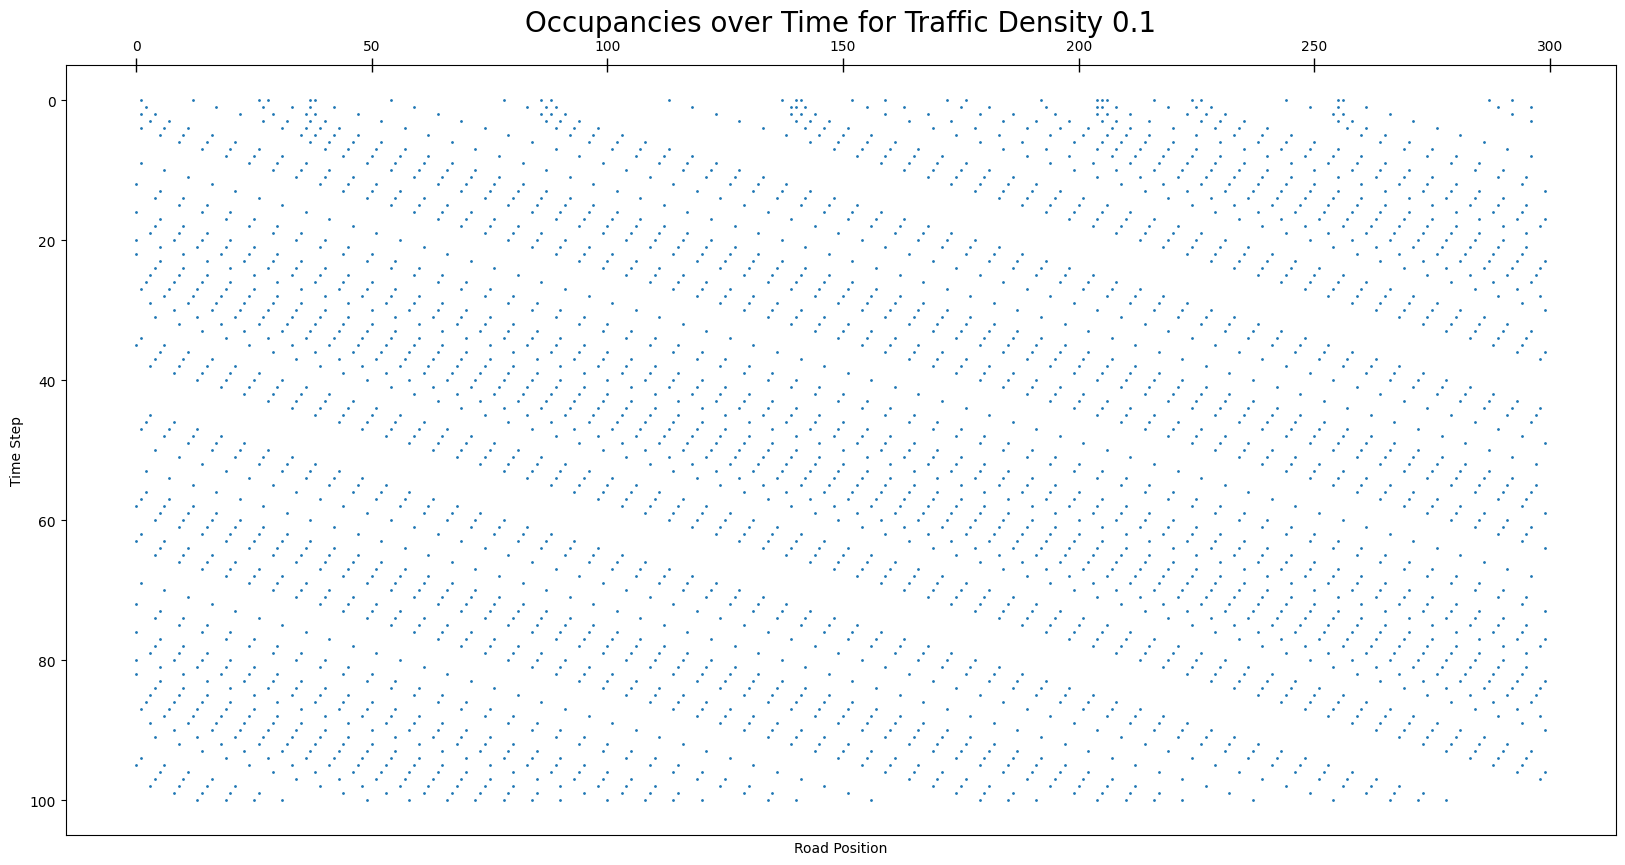
\includegraphics[width=0.75\linewidth]{assets/d0.1.png}
\end{figure}
\subsection{Density 0.25}
Graph
\begin{figure}[!h]
    \centering
    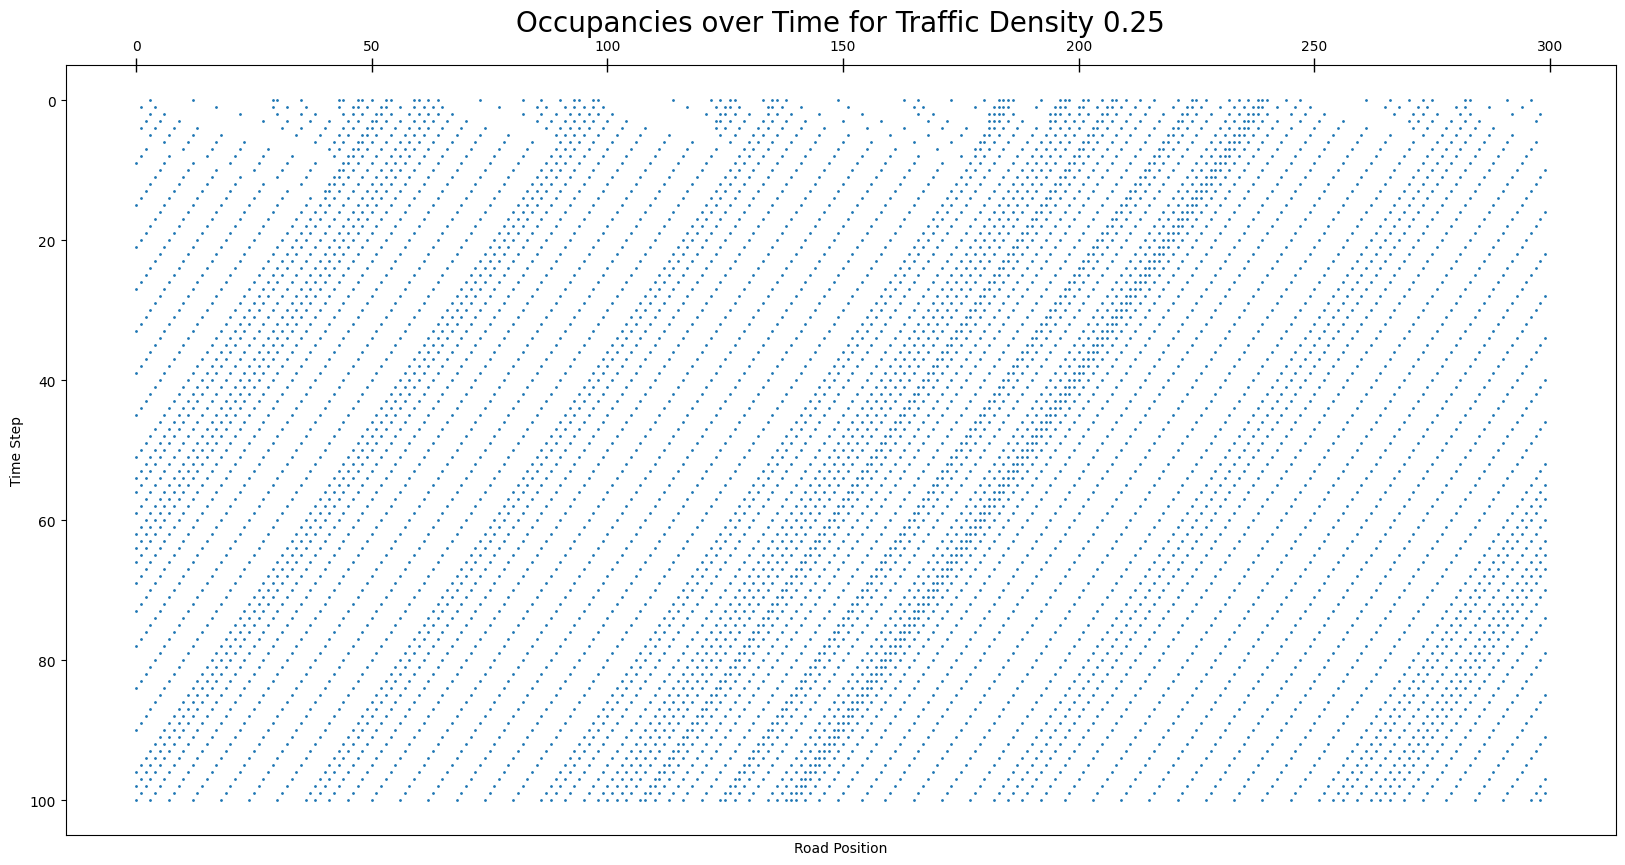
\includegraphics[width=0.75\linewidth]{assets/d0.25.png}
\end{figure}

\newpage
\subsection{Density 0.5}
\begin{figure}[!h]
    \centering
    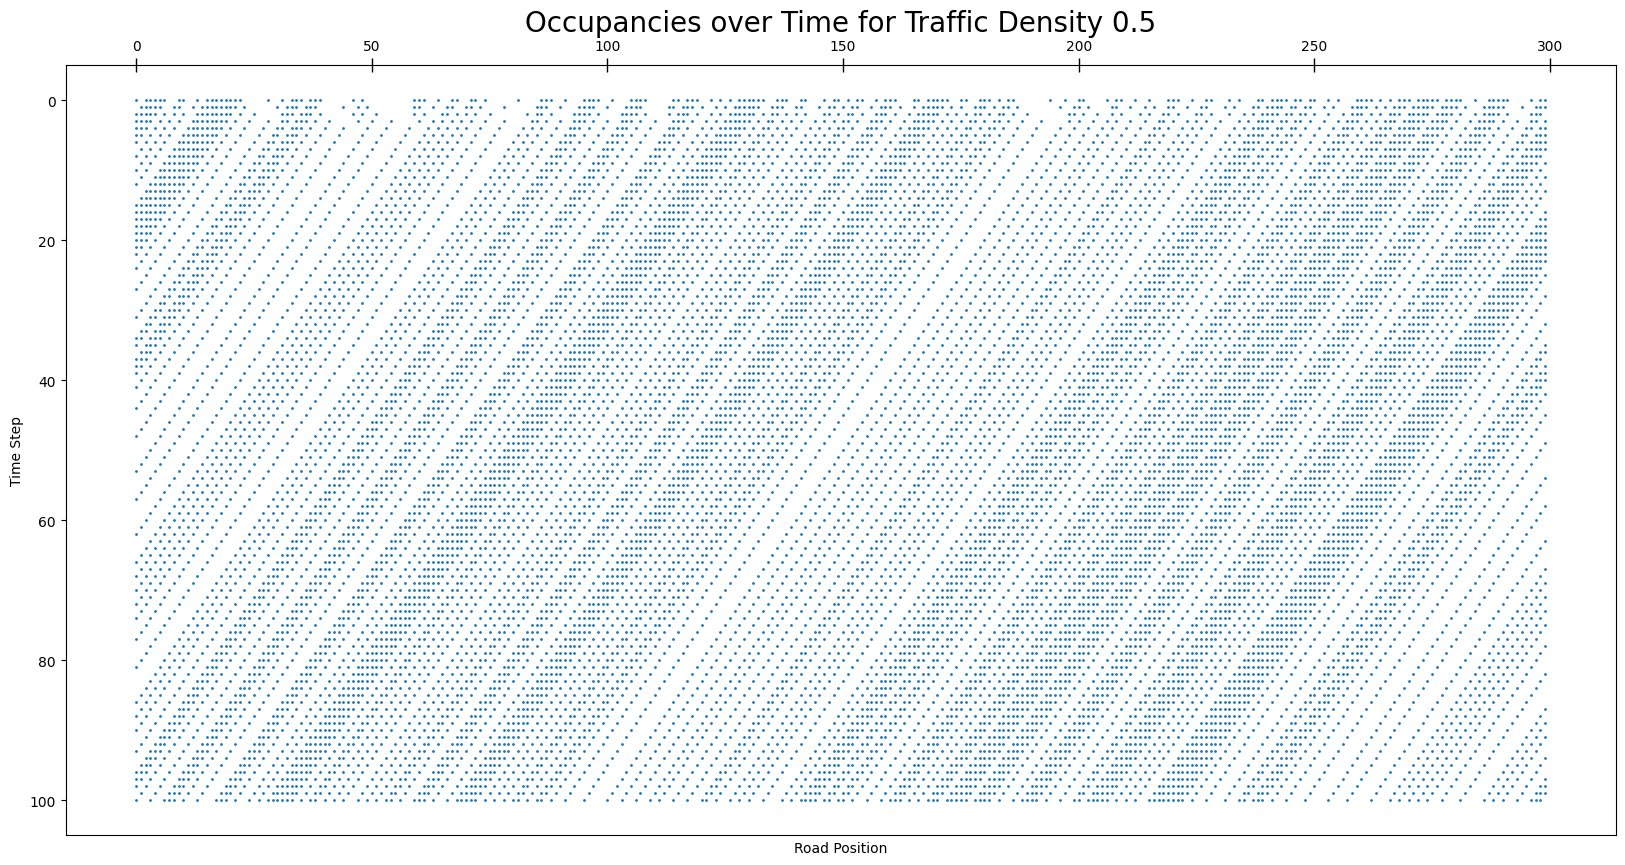
\includegraphics[width=0.75\linewidth]{assets/d0.5.png}
\end{figure}
\subsection{Density 0.8}
\begin{figure}[!h]
    \centering
    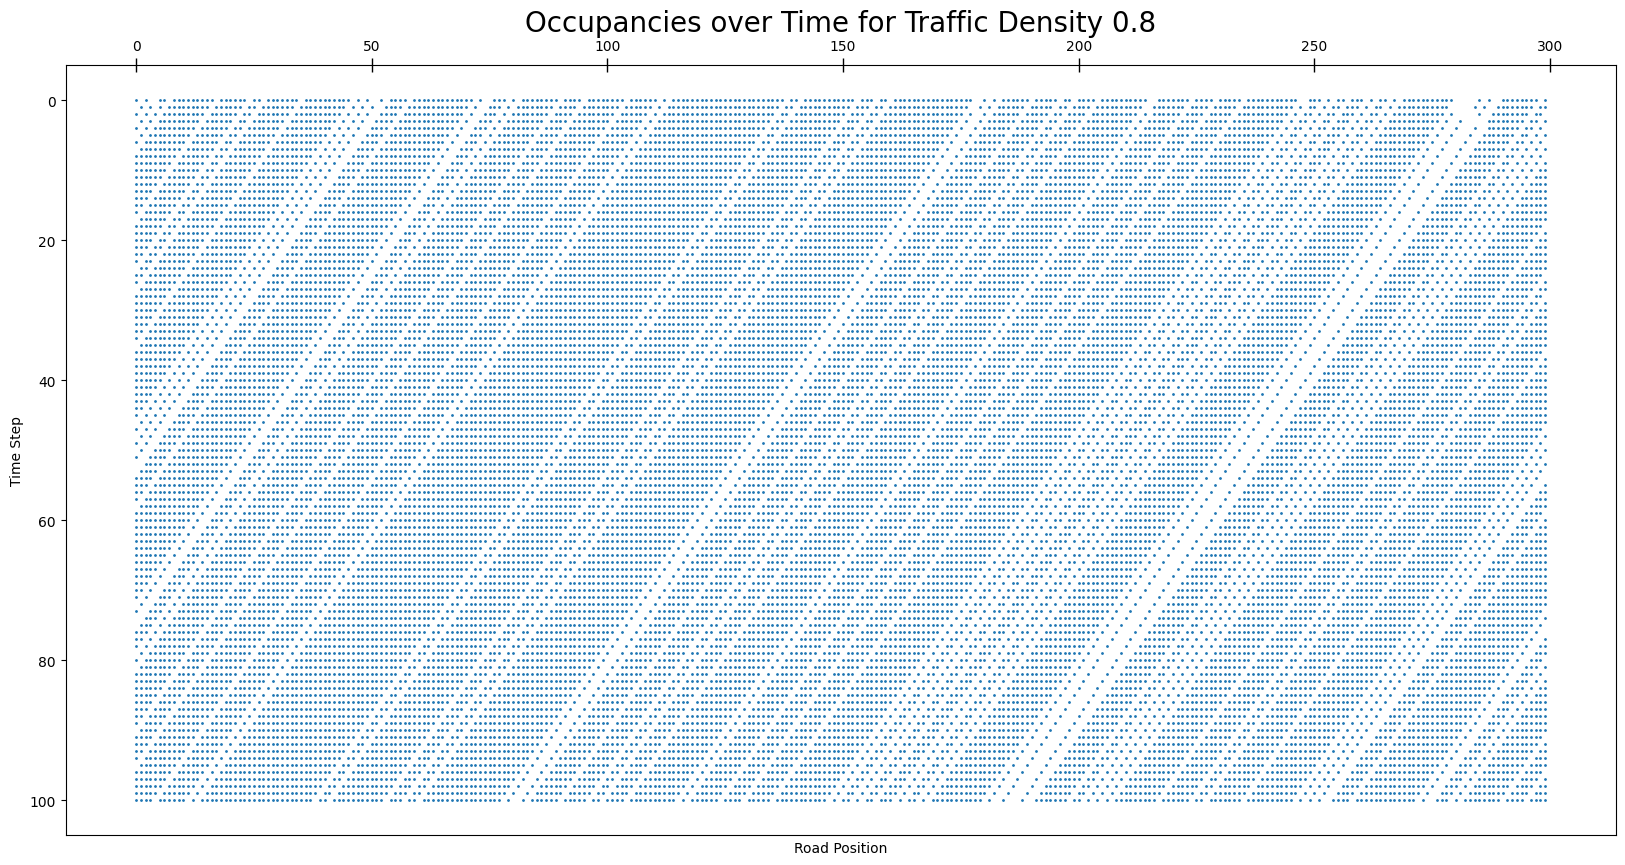
\includegraphics[width=0.75\linewidth]{assets/d0.8.png}
\end{figure}
\subsection{Written Questions}
\begin{enumerate}
    \item 
    \textbf{Verification of Implementation: } The TrafficSimulation class within the Jupyter notebook that is used provides a clear and concise implementation of a cellular automata model for traffic simulation, closely adhering to the principles and rules outlined in Algorithm 8.1 of the reading. This algorithm simulates the dynamics of vehicular movement on a single-lane road, where each vehicle's behavior is determined by three primary rules: acceleration, deceleration (to avoid collisions), and movement, taking into account the vehicle ahead. 
    
    In the initialization method of the TrafficSimulation class, the road is represented as a one-dimensional array, where each cell can either be empty (denoted by -1) or occupied by a car, with the car's current velocity as its value. This setup mirrors the cellular automata model's representation of space, where the road is discretized into cells that vehicles can occupy. The density parameter controls the initial distribution of cars on the road, with their velocities randomly assigned between 0 and $v_{\text{max}}$, reflecting the model's stochastic nature in vehicle speed at the start of the simulation.

    The update method within the class encapsulates the core logic for updating the state of the road based on the cellular automata rules. The acceleration step allows each vehicle to increase its speed by one unit, up to a maximum velocity $v_{\text{max}}$, embodying the model's attempt to simulate drivers' desire to move as fast as possible or up to the speed limit. The deceleration step ensures that vehicles adjust their speed to avoid colliding with the vehicle ahead, thereby maintaining a safe distance between cars. This is achieved by calculating the distance to the next car and adjusting the speed accordingly, ensuring the model's adherence to real-world driving behavior where safety is a major priority. Finally, the movement step translates the vehicles forward based on their updated velocities, actualizing the progression of traffic flow over discrete time steps.

    This implementation properly represents the cellular automata model's approach to simulating traffic, focusing on individual vehicle behaviors and their interactions to replicate the phenomena observed in real traffic systems, such as traffic jams and variations in flow density. By adhering to the specified algorithmic rules and incorporating stochastic elements in vehicle initialization, the model works to capture the complexity and variability inherent in traffic dynamics.

    \item 
    \textbf{Comparison of Plots With Different Occupancies: } 
    First, we'll start with a brief discussion of observations in the different plots: 
    \begin{enumerate}
        \item 
        Low Density (0.1): The plot shows vehicles widely spaced, and there appear to be no traffic jams forming. The vehicles move forward mostly unhindered, maintaining their speeds or accelerating up to the maximum speed limit. This reflects the free-flow phase, where the low density allows vehicles to move at or near $v_\text{max}$ without significant interactions.

        \item
        Medium Density (0.25): At this increased density, we see more vehicles on the road. Still, they seem to continue moving smoothly, albeit with slight variations in speeds likely due to occasional braking. This state suggests a stable traffic flow, possibly at the beginning stages where interactions are more frequent, but traffic jams are not yet forming, consistent with the transition from free flow to congested traffic.

        \item
        High Density (0.5): This plot begins to show characteristics of congested traffic. The increased vehicle count causes more frequent interactions, leading to a mix of slow-moving traffic and pockets of higher-speed movement. Vehicles are closer together, indicating a shift towards higher-density traffic behavior where the flow becomes unstable.

        \item
        Very High Density (0.8): The plot illustrates a heavily congested road. The high density leads to numerous interactions, with vehicles frequently slowing down or stopping, showing patterns typical of traffic jams. This situation closely resembles stop-and-go waves, a phenomenon characteristic of high-density traffic flow, where vehicles frequently alternate between moving and stationary states.
    \end{enumerate}

    Chapter 8.2 indicates that for lower densities, traffic behaves in a free-flow manner, with vehicles largely unaffected by the presence of others. As density increases, traffic flow remains stable until a critical density is reached, beyond which traffic jams can form spontaneously. The provided plots corroborate these claims, showing a clear transition from free-flow at low densities to more complex, interactive behavior at higher densities, leading to the formation of traffic jams. 

    The model's predictions are visualized in these plots, where at low densities (0.1 and 0.25), the traffic is well below the critical density, resulting in a relatively stable flow. As the density approaches the critical threshold (0.5), we begin to see the instability and fluctuations in speed indicative of the onset of congested traffic. At very high densities (0.8), the simulations depict sustained traffic jams, with some vehicles forced to a complete halt, aligning with the assertion that beyond the critical density, traffic flow becomes unstable and jams become persistent.

    That being said, the simulation results do show a steady traffic situation occurs after a phase of adjustments initially - but this is not really true to what we see in the real world with regards to traffic. While the model is correct in that greater densities beyond a critical point will cause traffic build-up, the model doesn't properly capture real-life driving behaviors on the streets, warranting an extension of this initial model to simulate more realistic behavior, like Section 8.2 concludes. This will be elaborated on further in later sections of this report. 
\end{enumerate}

\newpage
\section{Task 1.2 - Stochastic Behavior}
\subsection{Density 0.1}
\begin{figure}[!h]
    \centering
    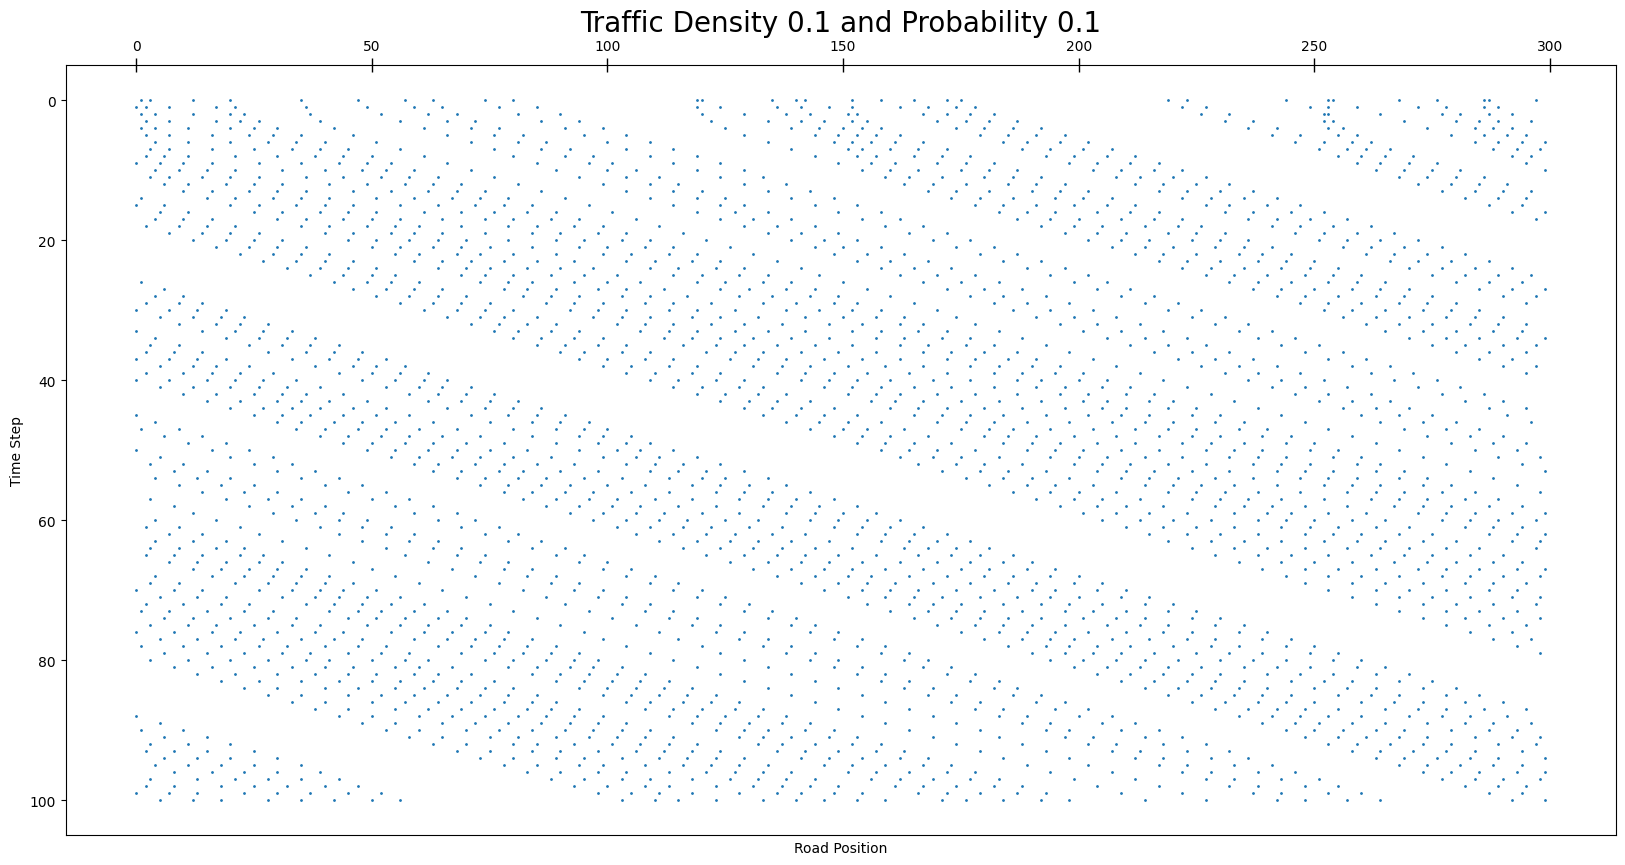
\includegraphics[width=0.70\linewidth]{assets/d0.1p0.1.png}
\end{figure}

\begin{figure}[!h]
    \centering
    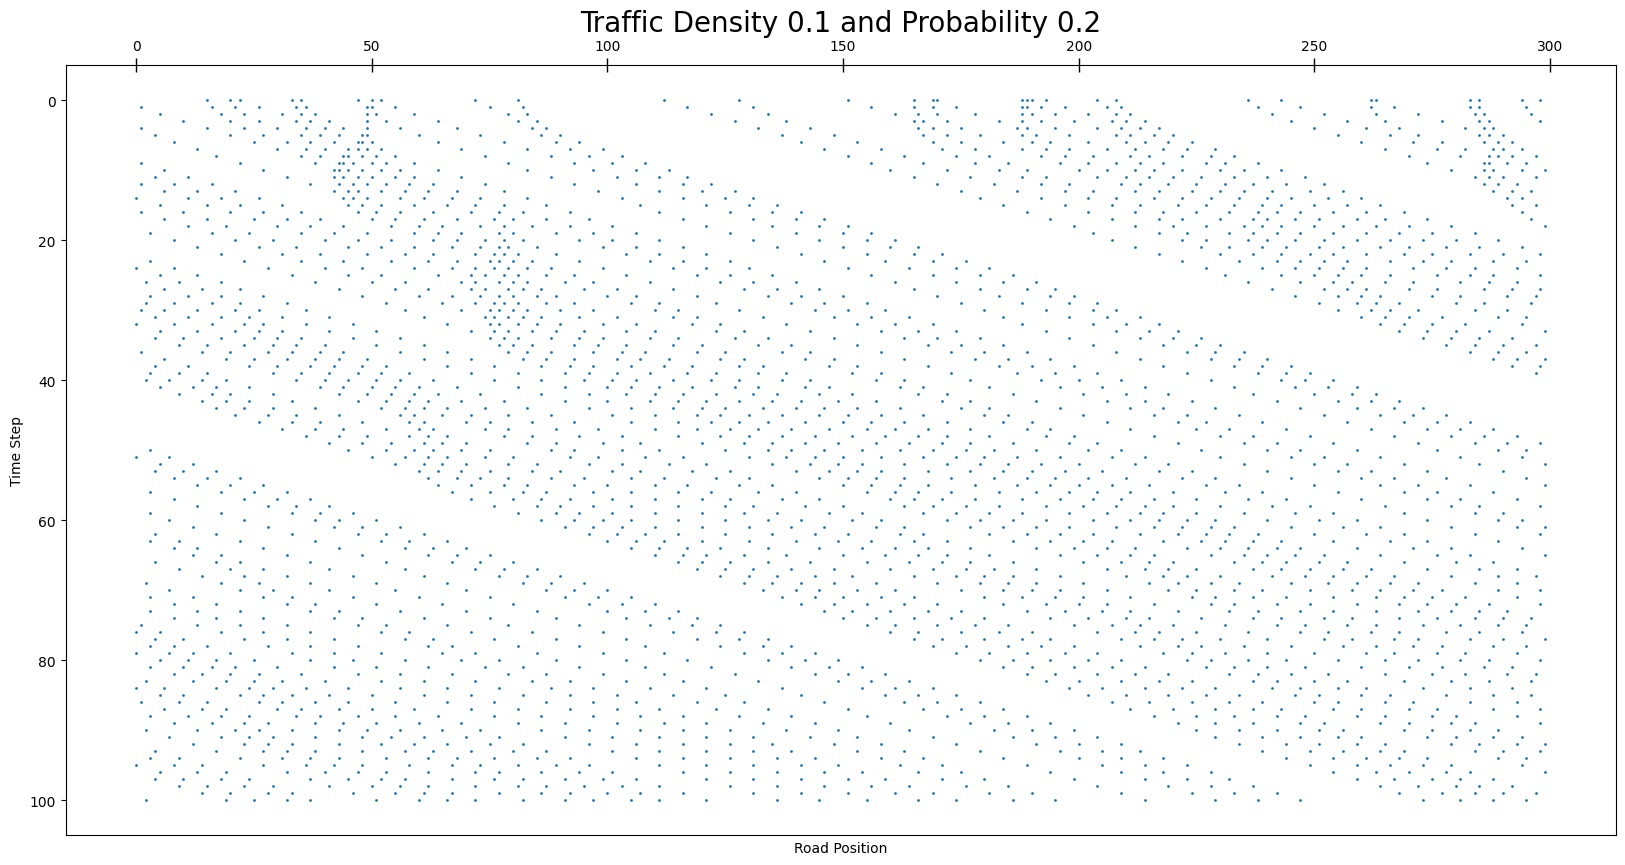
\includegraphics[width=0.70\linewidth]{assets/d0.1p0.2.png}
\end{figure}

\begin{figure}[!h]
    \centering
    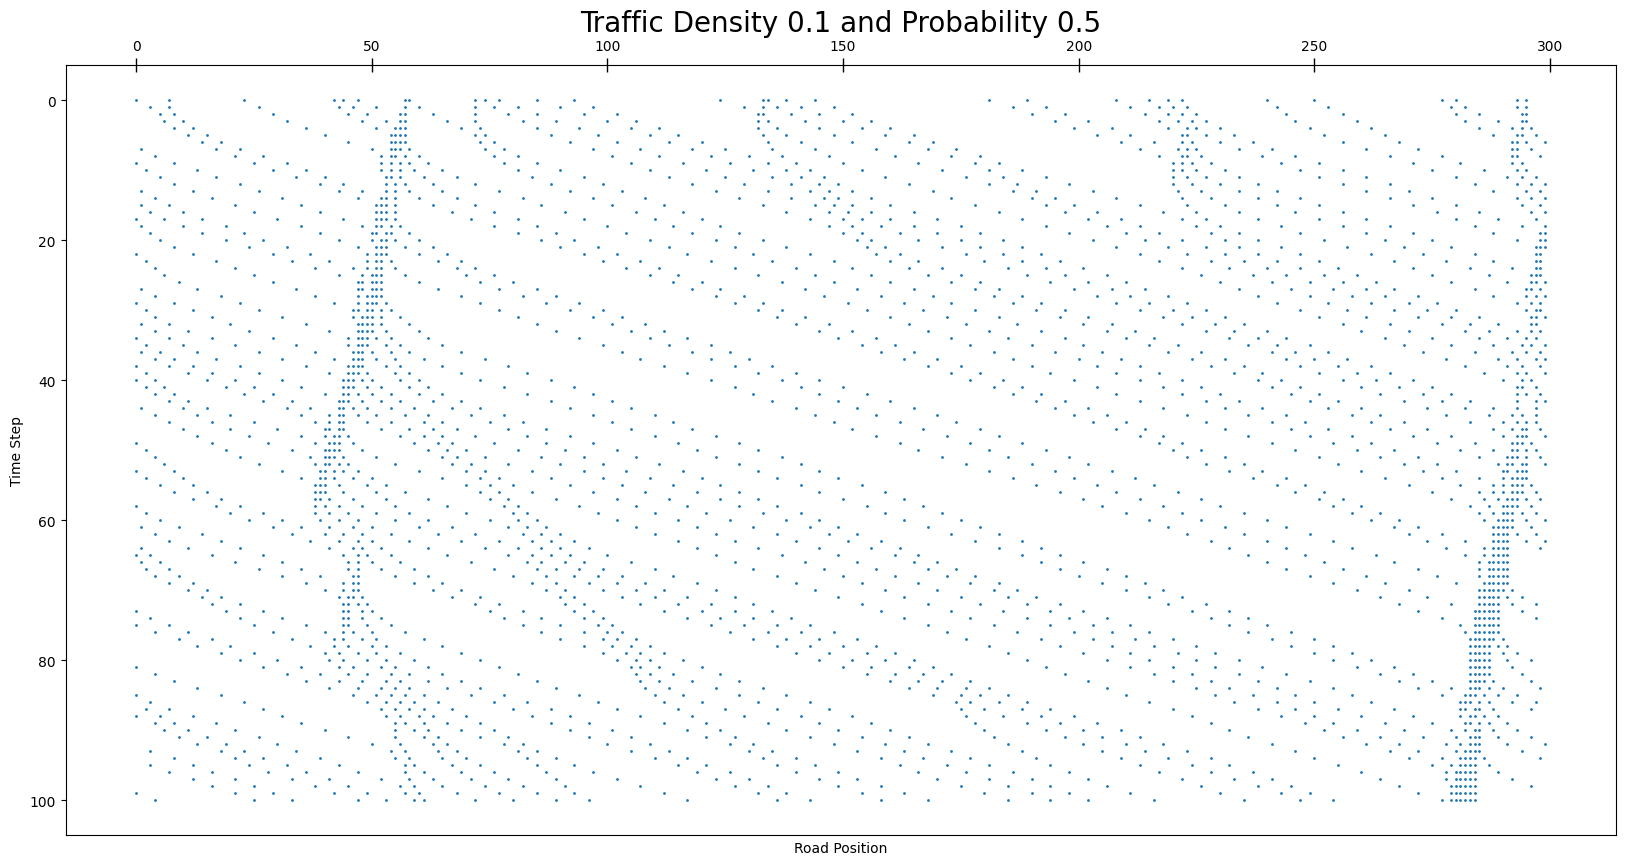
\includegraphics[width=0.70\linewidth]{assets/d0.1p0.5.png}
\end{figure}

\newpage
\subsection{Density 0.25}
\begin{figure}[!h]
    \centering
    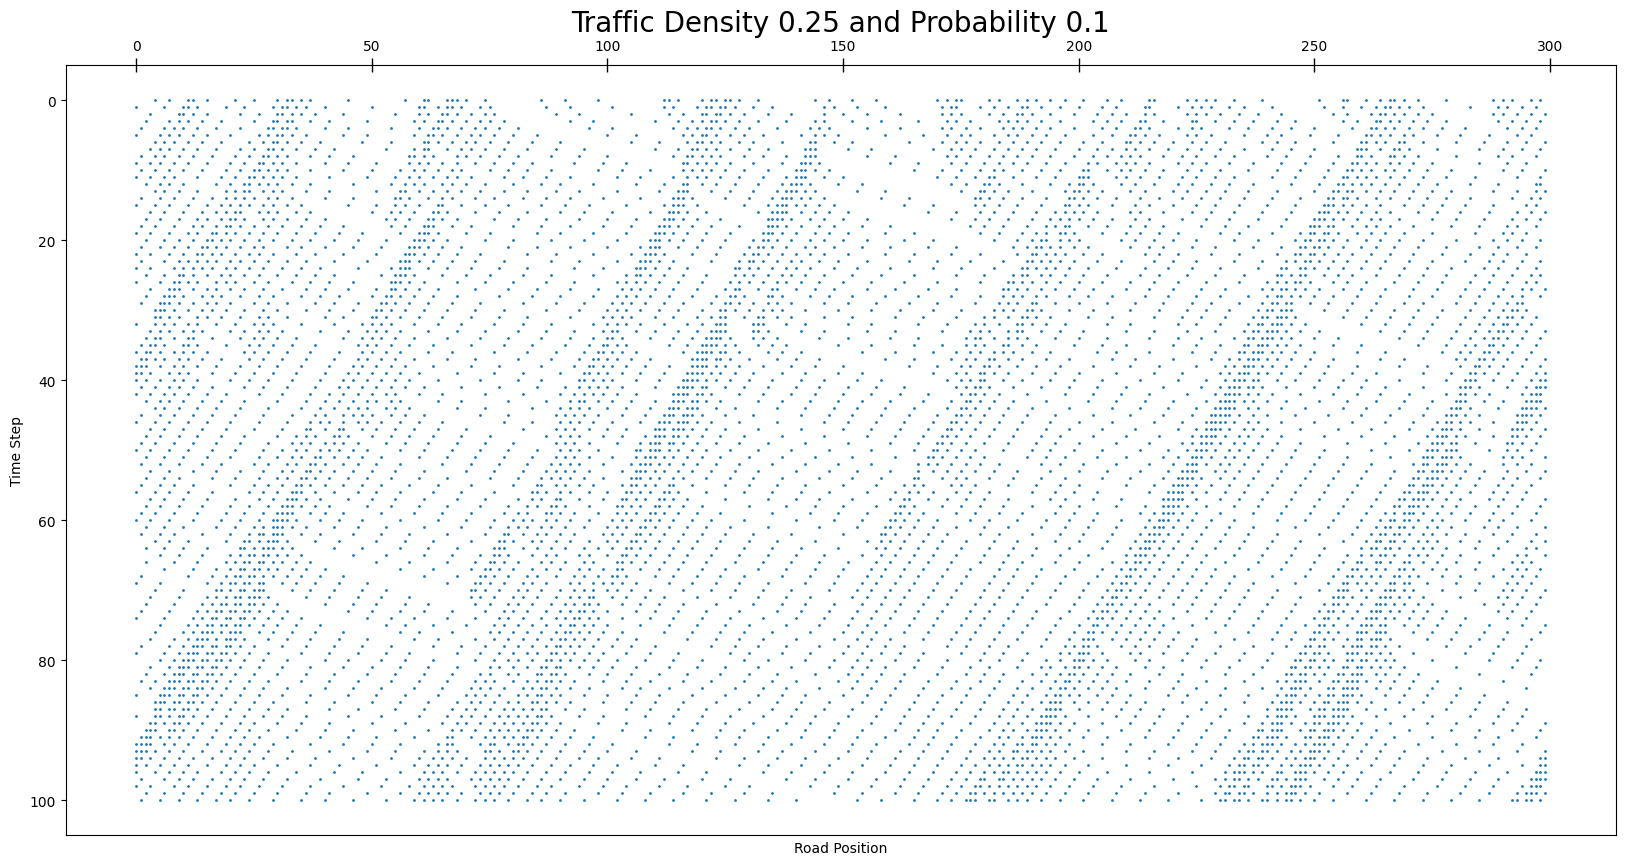
\includegraphics[width=0.70\linewidth]{assets/d0.25p0.1.png}
\end{figure}

\begin{figure}[!h]
    \centering
    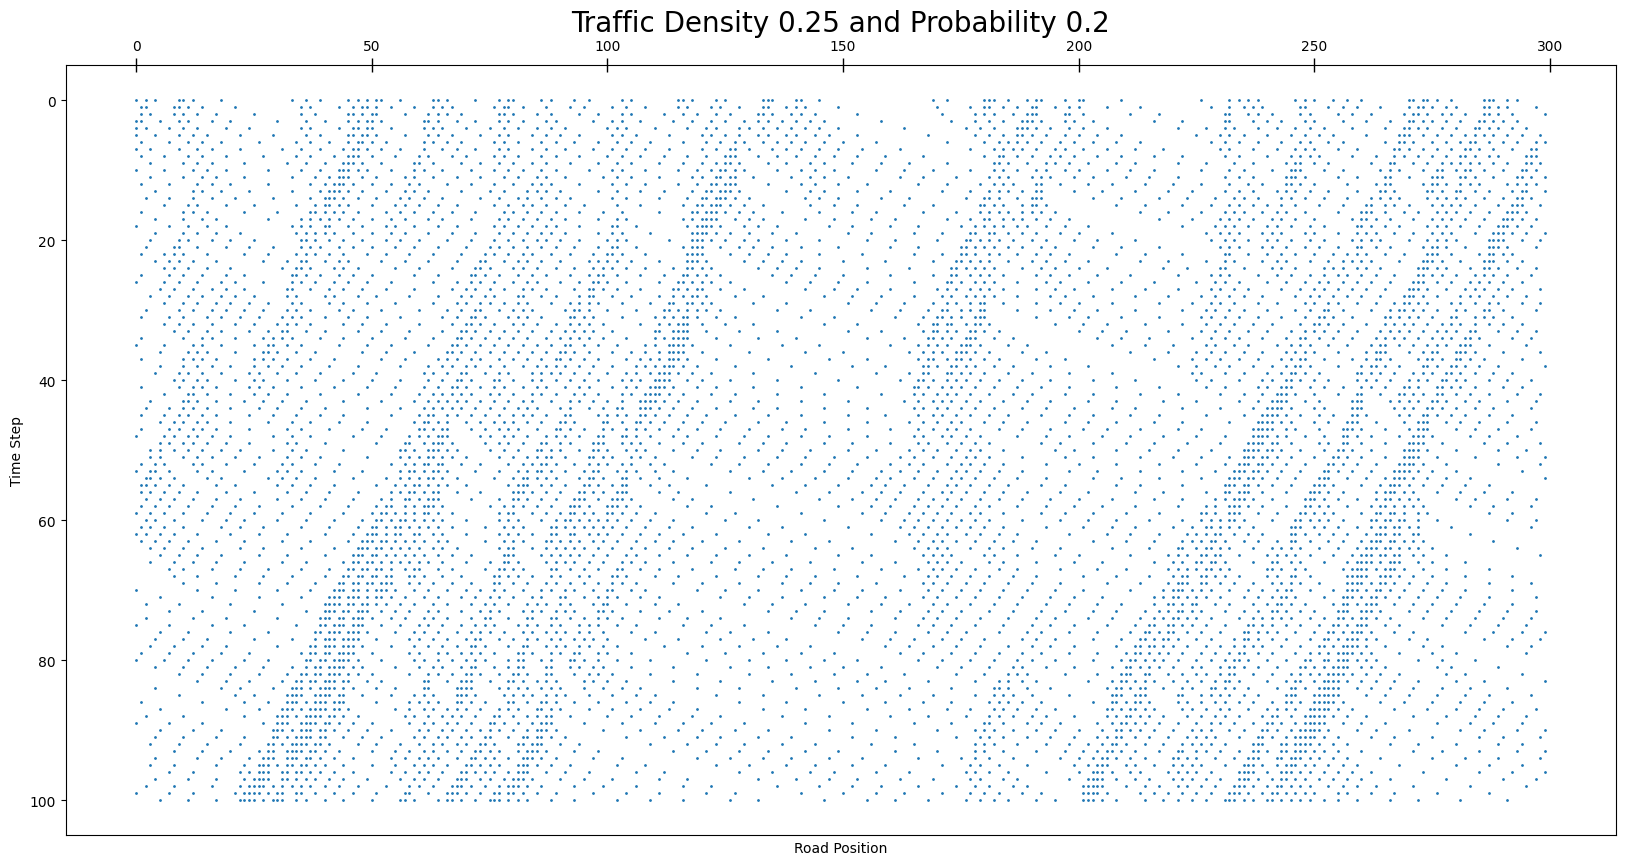
\includegraphics[width=0.70\linewidth]{assets/d0.25p0.2.png}
\end{figure}

\begin{figure}[!h]
    \centering
    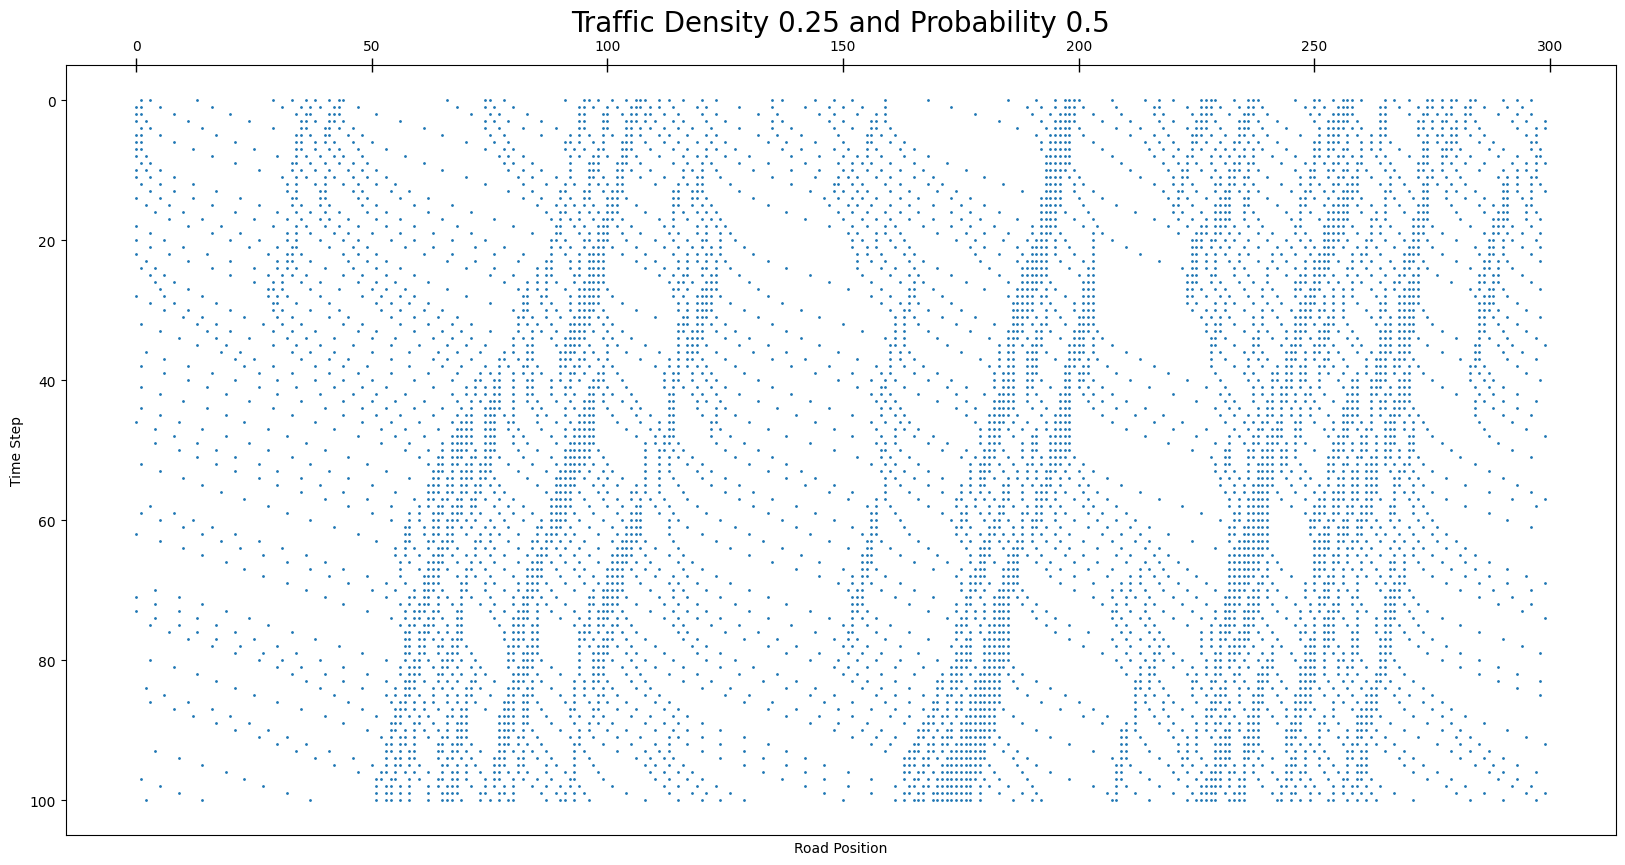
\includegraphics[width=0.70\linewidth]{assets/d0.25p0.5.png}
\end{figure}

\newpage
\subsection{Density 0.5}
\begin{figure}[!h]
    \centering
    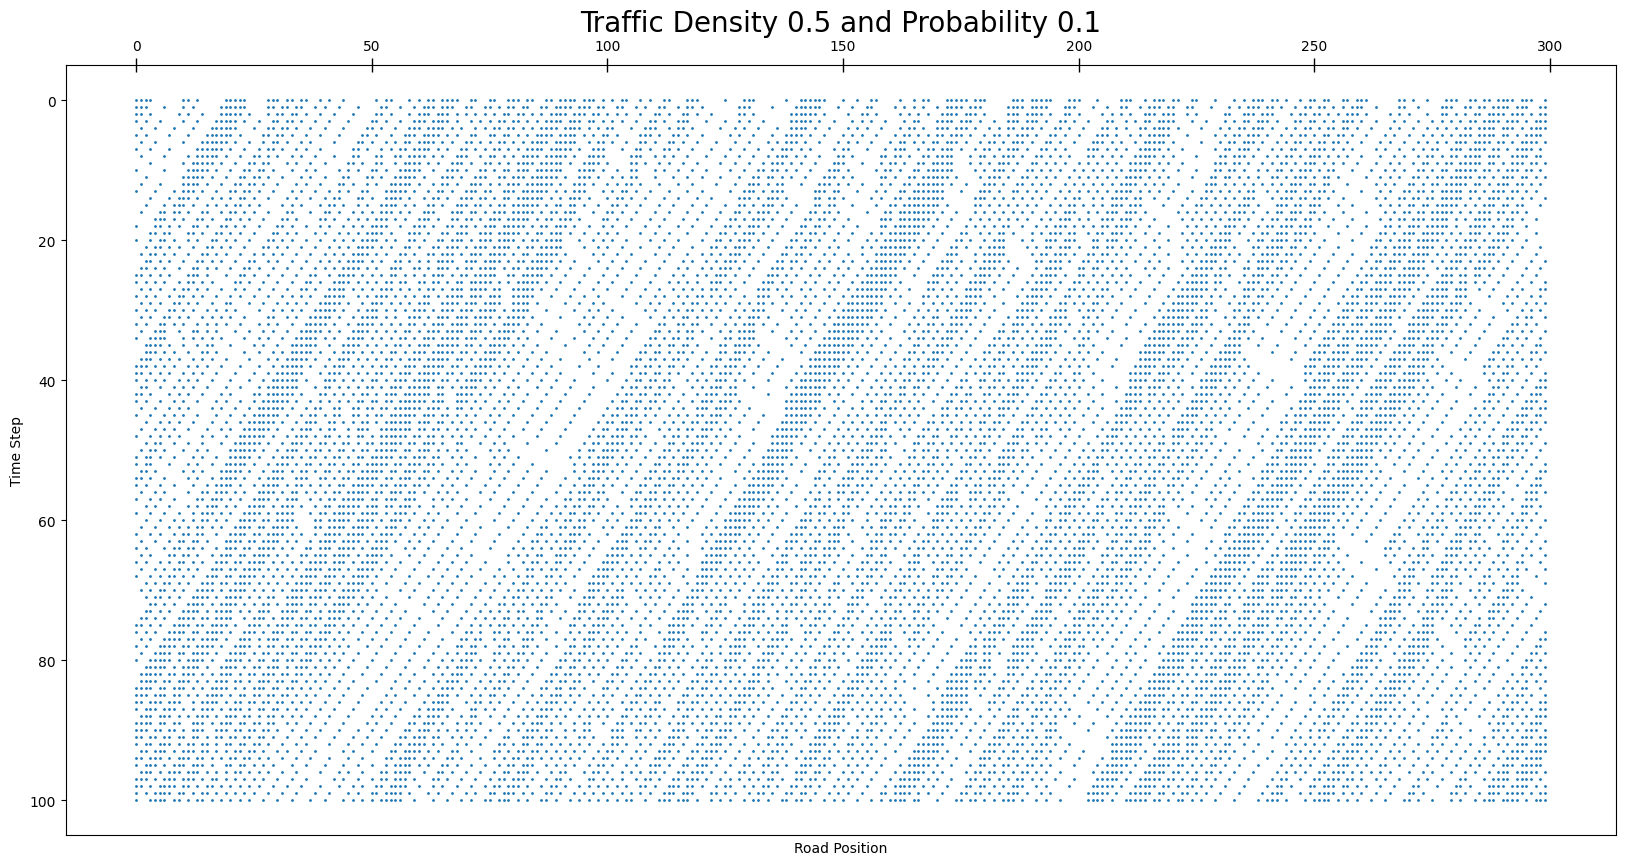
\includegraphics[width=0.70\linewidth]{assets/d0.5p0.1.png}
\end{figure}

\begin{figure}[!h]
    \centering
    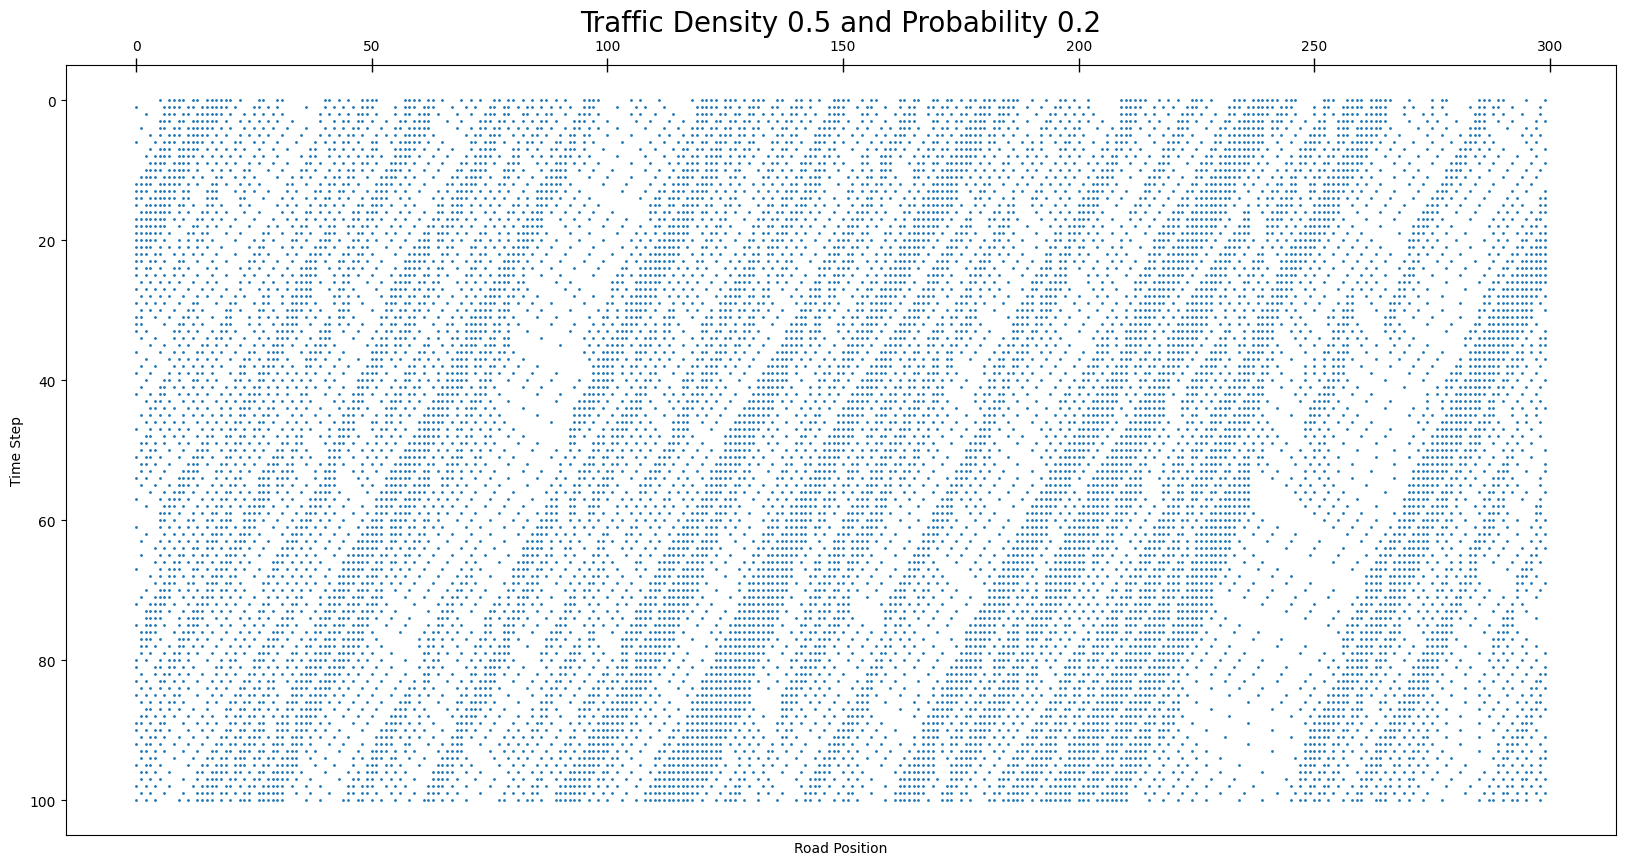
\includegraphics[width=0.70\linewidth]{assets/d0.5p0.2.png}
\end{figure}

\begin{figure}[!h]
    \centering
    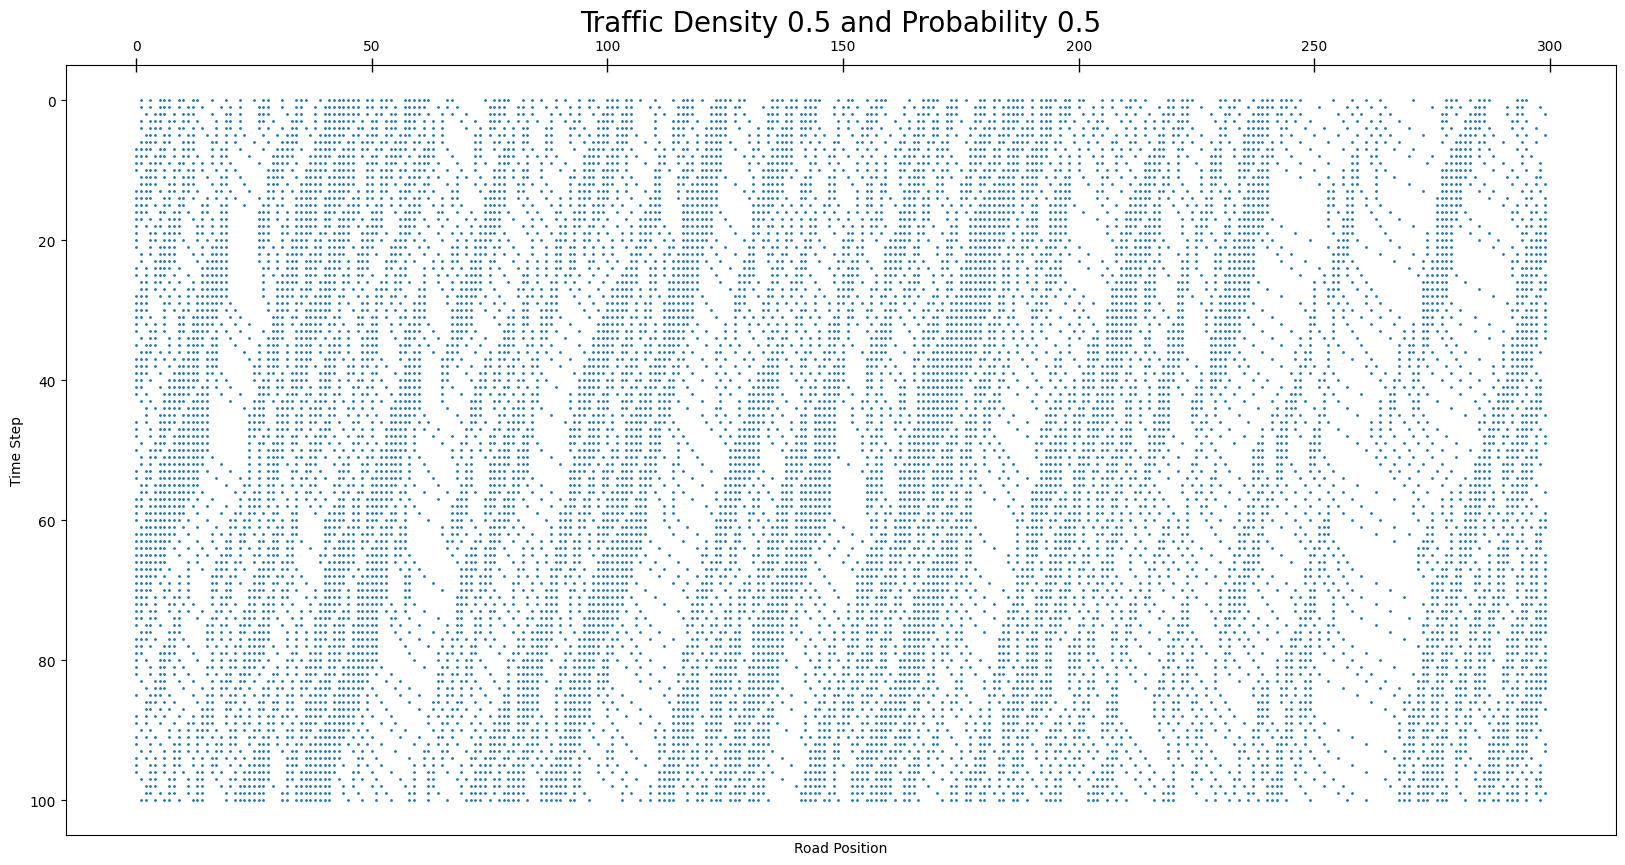
\includegraphics[width=0.70\linewidth]{assets/d0.5p0.5.png}
\end{figure}

\newpage
\subsection{Density 0.8}
\begin{figure}[!h]
    \centering
    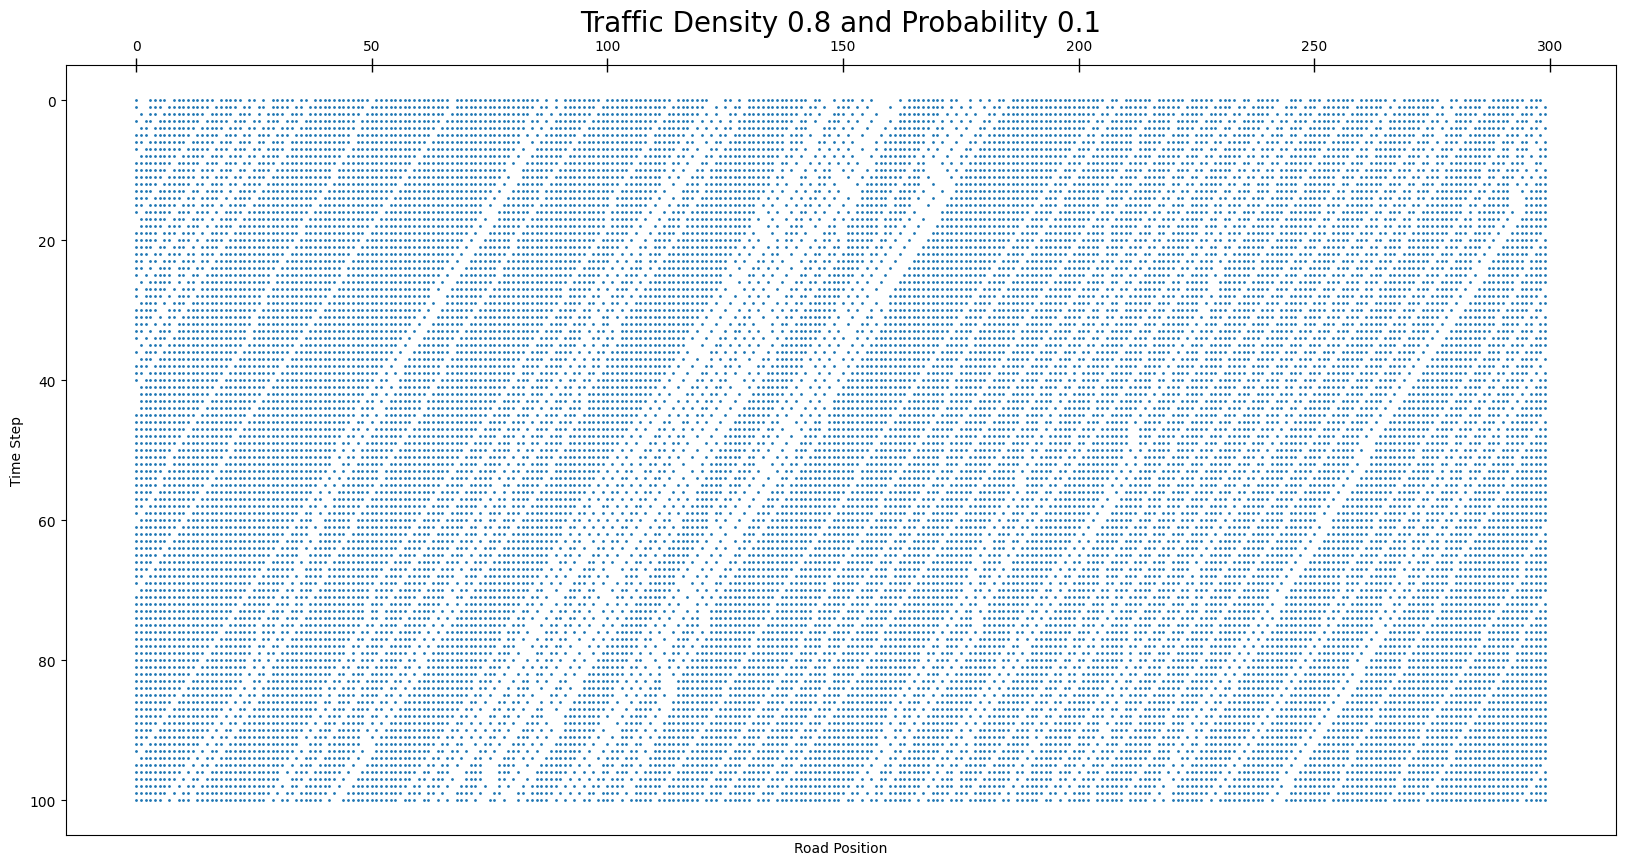
\includegraphics[width=0.70\linewidth]{assets/d0.8p0.1.png}
\end{figure}

\begin{figure}[!h]
    \centering
    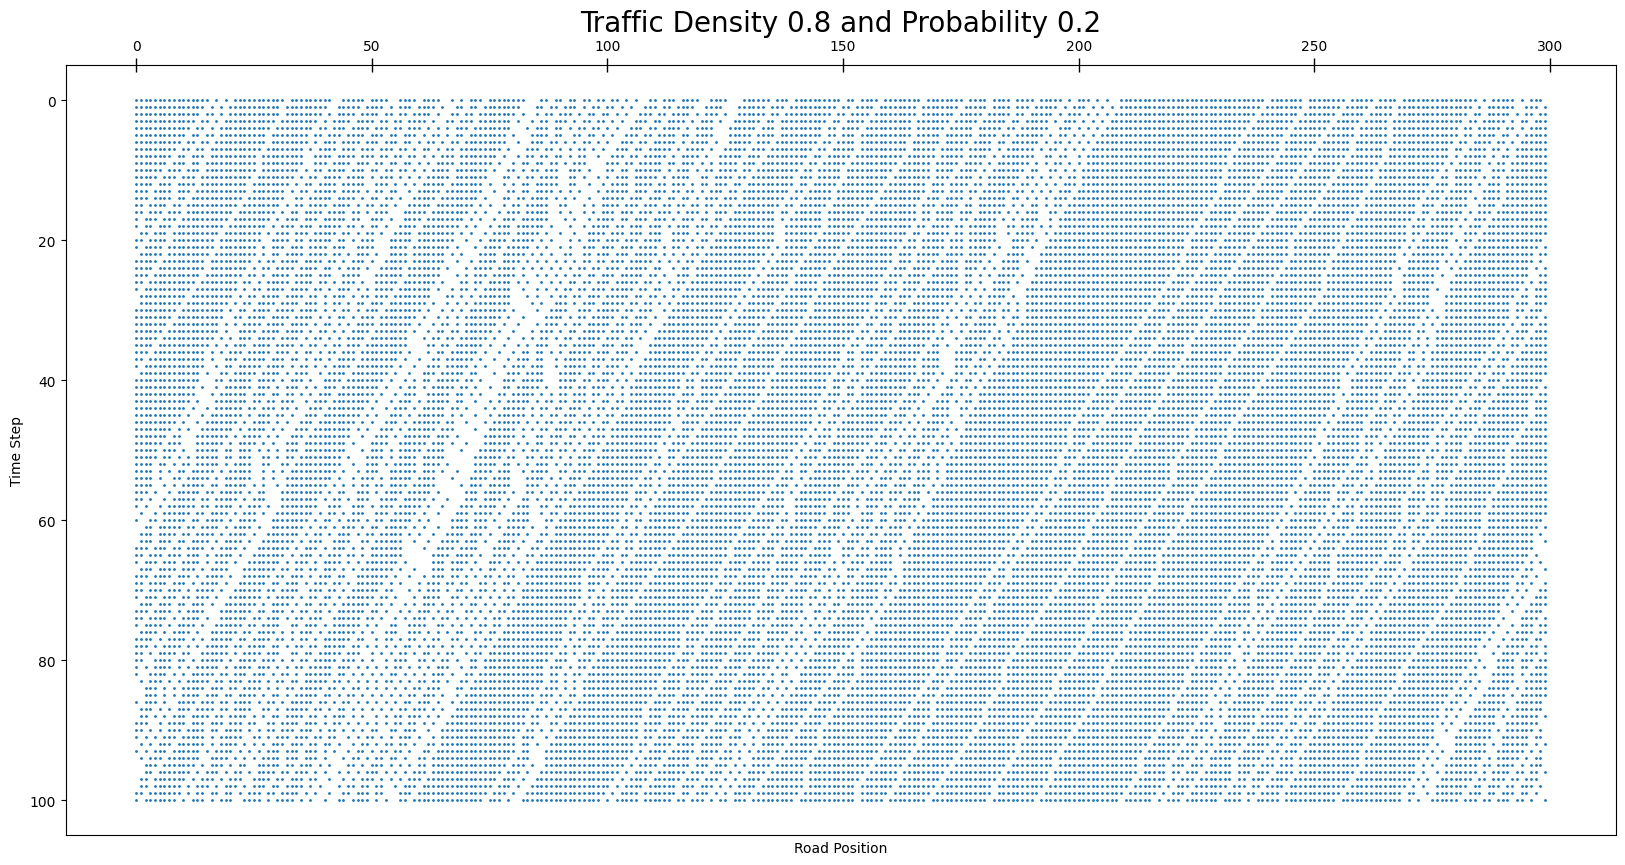
\includegraphics[width=0.70\linewidth]{assets/d0.8p0.2.png}
\end{figure}

\begin{figure}[!h]
    \centering
    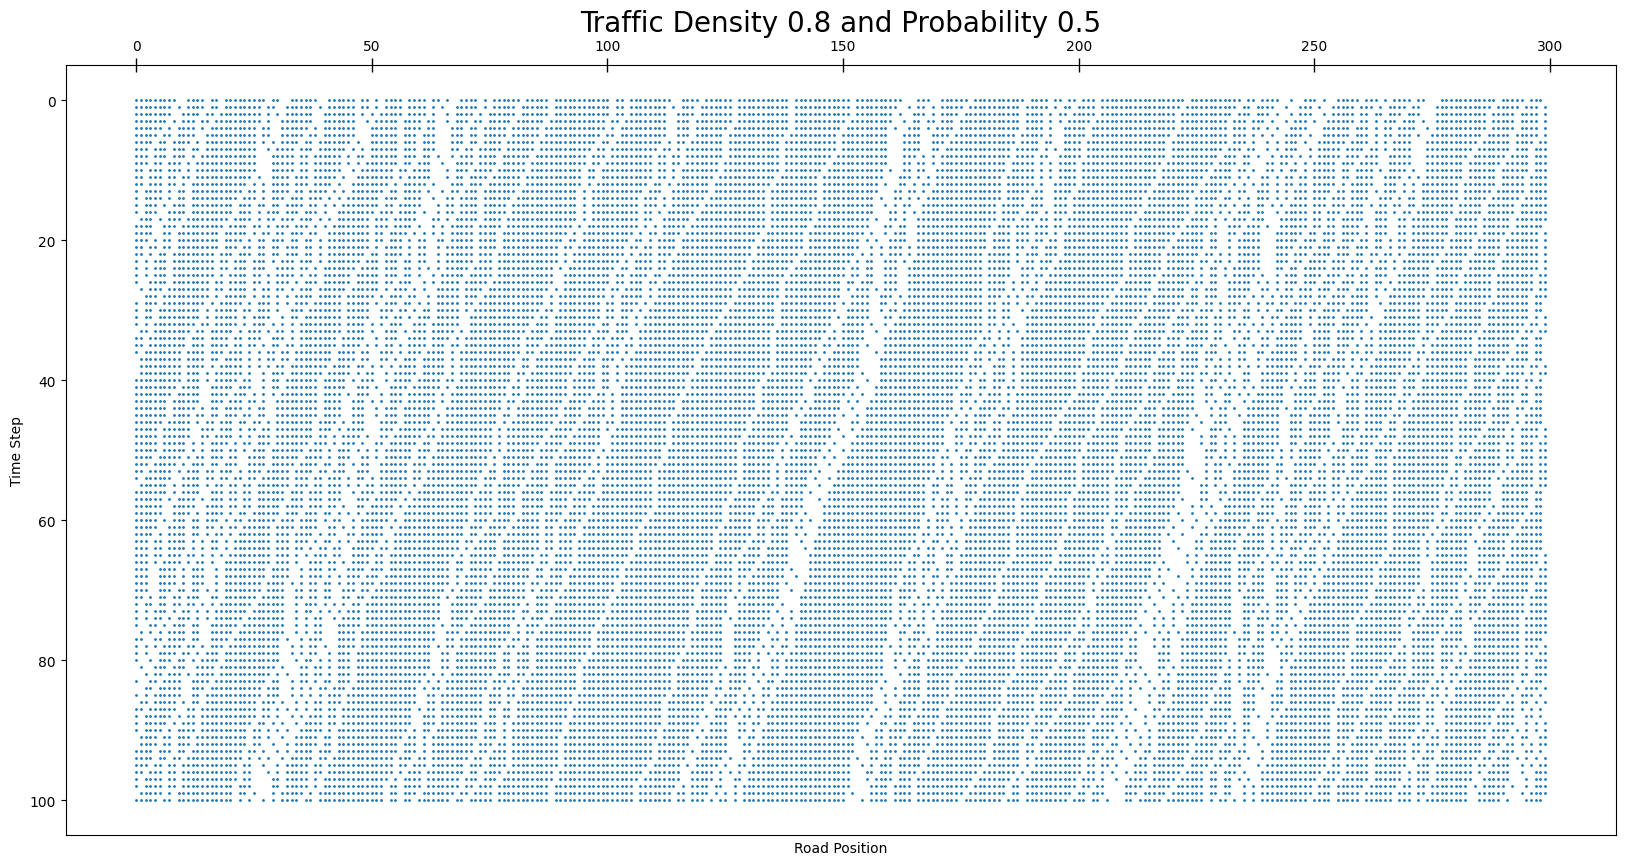
\includegraphics[width=0.70\linewidth]{assets/d0.8p0.5.png}
\end{figure}

\subsection{Written Questions}
\begin{enumerate}
    \item 
    \textbf{Comparison of Task 1 with Added Dally Factor:} The inclusion of the dally factor introduces an element of randomness into each car's behavior, simulating the natural variability (a human factor) in human driving (e.g. delayed reactions, distractions, variations in styles of driving, etc.). This factor changes a car's velocity with a certain probability (in this case, $p = 0.2$, meaning there's a 20\% chance in each time step that a car will randomly slow down by one unit of velocity). 
    
    The plot for the traffic density of 0.1 without the dally factor shows a regular, predictable pattern of traffic flow - the cars appear to accelerate to $v_\text{max}$ and maintain it consistently over time, without spontaneous reductions in speed. 
    
    Introducing the dally factor changes this behavior. Despite the overall density remaining the same, the cars no longer maintain a constant velocity. Instead, we begin to see instances where vehicles randomly slow down, deviating from the uniform motion observed in Task 1. This leads to more variability in the flow of traffic, and we can see patterns that showcase the beginnings of traffic disturbances over time. 

    The most striking difference between the two plots (where density = 0.1) is the variability in the speed of the cars when the dally factor is introduced. Without the dally factor, the traffic appears to be more idealized, while the dally factor brings the simulation closer towards real-world conditions by including the unpredictable nature of human driving behaviors. The plot including the dally factor (density = 0.1, p = 0.2) shows that fluctuations in vehicle speeds can occur due to the dally factor. These fluctuations are a crucial aspect of modeling traffic because they can lead to the formation of traffic jams, even in seemingly free-flow conditions, as drivers react variably. 

    \item 
    \textbf{Comparison of Dally Factor Experiment to Task 1 and Reading:} Incorporating the dally, as seen in the new simulation plots (shown previously in this section of the document) better showcases the impact of human behavior on traffic flow than beyond just a variable occupancy of roads. Below is a comparison of simulations from Task 1 and simulations including dally factor. 
    \begin{itemize}
        \item 
        Starting with simulations having low density and various dally factors - the plots with a dally factor show more variation in vehicle speed and positions over time than the plot without any dally factor. The inclusion of the dally factor creates sporadic braking, which can be seen as disruptions in the otherwise smooth diagonal lines of the original low density plot. These disruptions become more pronounced as the dally factor increases, indicating that higher probabilities of dallying, or inconsistent driving (due to various human factors), introduce more frequent and significant disturbances in traffic flow. 

        \item 
        Continuing on to compare simulations having medium density (0.25, 0.5) with varying dally factors - at a medium density, the plots with dally factors show the beginning of more extensive traffic disturbances. Compared to the original plots without the dally factor and medium density, the added randomness creates greater instances of slower movement and potential for jam formations. This effect intensifies with a higher dally probability, as seen with the greater jams illustrated in the figures where density = 0.25 or 0.5, and $p = 0.5$. This shows that even moderate densities can lead to unstable traffic flow when driver behavior is more variable or erratic. 

        \item 
        At high density, the simulations with the dally factor depict a more realistic and complex simulation of traffic flow. The inherent variability due to the dally factor results in various stop-and-go waves. When contrasted with the high-density plot that includes no dally factor, the randomness results in more realistic congestion patterns that reflect actual traffic scenarios more closely. 
    \end{itemize}

    Comparing these results to the figures in Chapter 8 (specifically figs. 8.5-8.7) reveals the model's improved capability to mimic real-world traffic conditions. The dally factor introduces elements that lead to emergent phenomena like phantom traffic jams, like in figure 8.5, where hams occur and dissolve without any cause other than the variability in driver behavior. Figure 8.7 demonstrates longer and more persistent jams at critical density, a factor that also becomes apparent in the high density simulations with a dally factor. As $p$ increases, the simulations start to closely resemble the patterns observed in the figures from Chapter 8 of the provided reading with traffic jams that are not only longer and more persistent but also more sporadic. 

    In low-density environments, the original model without the dally factor might suffice as vehicles are less likely to interact. However, as density increases, the interactions become more critical, and the randomness introduced by the dally factor helps better capture the nuances of traffic behavior.

    The key takeaway is that the dally factor enhances the cellular automata model by capturing the spontaneous formation and dissipation of traffic jams. This addition makes the model more robust and adaptable to different traffic scenarios and occupancies (densities). 
    
    
\end{enumerate}

\newpage
\section{Question 1.3}
\subsection{Fundamental Diagram Analysis \& Summary}
Fundamental diagrams are useful in the context of modeling traffic flow, as it represents the relationship between the flow of traffic and the density of traffic. To create a fundamental diagram of actual road traffic, fundamental diagram points need to be recorded with measurements that cover different traffic situations. To determine the flow of traffic, we would need to measure the number of vehicles that pass a point (or, a measuring station) during a certain time interval. \\ \\
Practically speaking, measuring the density for a fundamental diagram is a bit more complex in the rea world. We'd need to determine the number of vehicles on a section of the road of a specified length at a point in time of the measurement. This can be achieved by taking photographs and either manually or automatically counting vehicles. An alternative approach is to determine the number of vehicles entering and leaving a road - if the road has been empty at the beginning, the number of vehicles can be computed and the local density can be approximated. This approach can be useful for a simulation. \\ \\
The fundamental diagram is usually represented with a scatter plot (like in the provided reading) to compare density with flow of traffic. Generally speaking, we can divide up a fundamental diagram into regions that represent the following: 
\begin{itemize}
    \item 
    \textbf{Free flow:} traffic density is low, allowing vehicles to travel at their desired speeds; flow increases linearly with density, and speed of vehicles stays relatively constant.

    \item 
    \textbf{Congested flow:} As density increases, the space between vehicles decreases, causing them to change their speed for aversion and safety purposes; flow reaches its maximum capacity, and the speed begins to decrease.

    \item 
    \textbf{Jammed flow:} When the density becomes too great, the flow will decrease, causing slow speeds or full stops for vehicles; the road becomes highly congested, and the speed will drop.
\end{itemize}
\subsection{Fundamental Diagram Implementation Results}
A reconstruction of Figure 8.9 is shown below. Our implementation of the simulations to generate the plot can be found in the Jupyter Notebook in our repository included in the submission (shared with the instructional team).

\begin{figure}[!h]
    \centering
    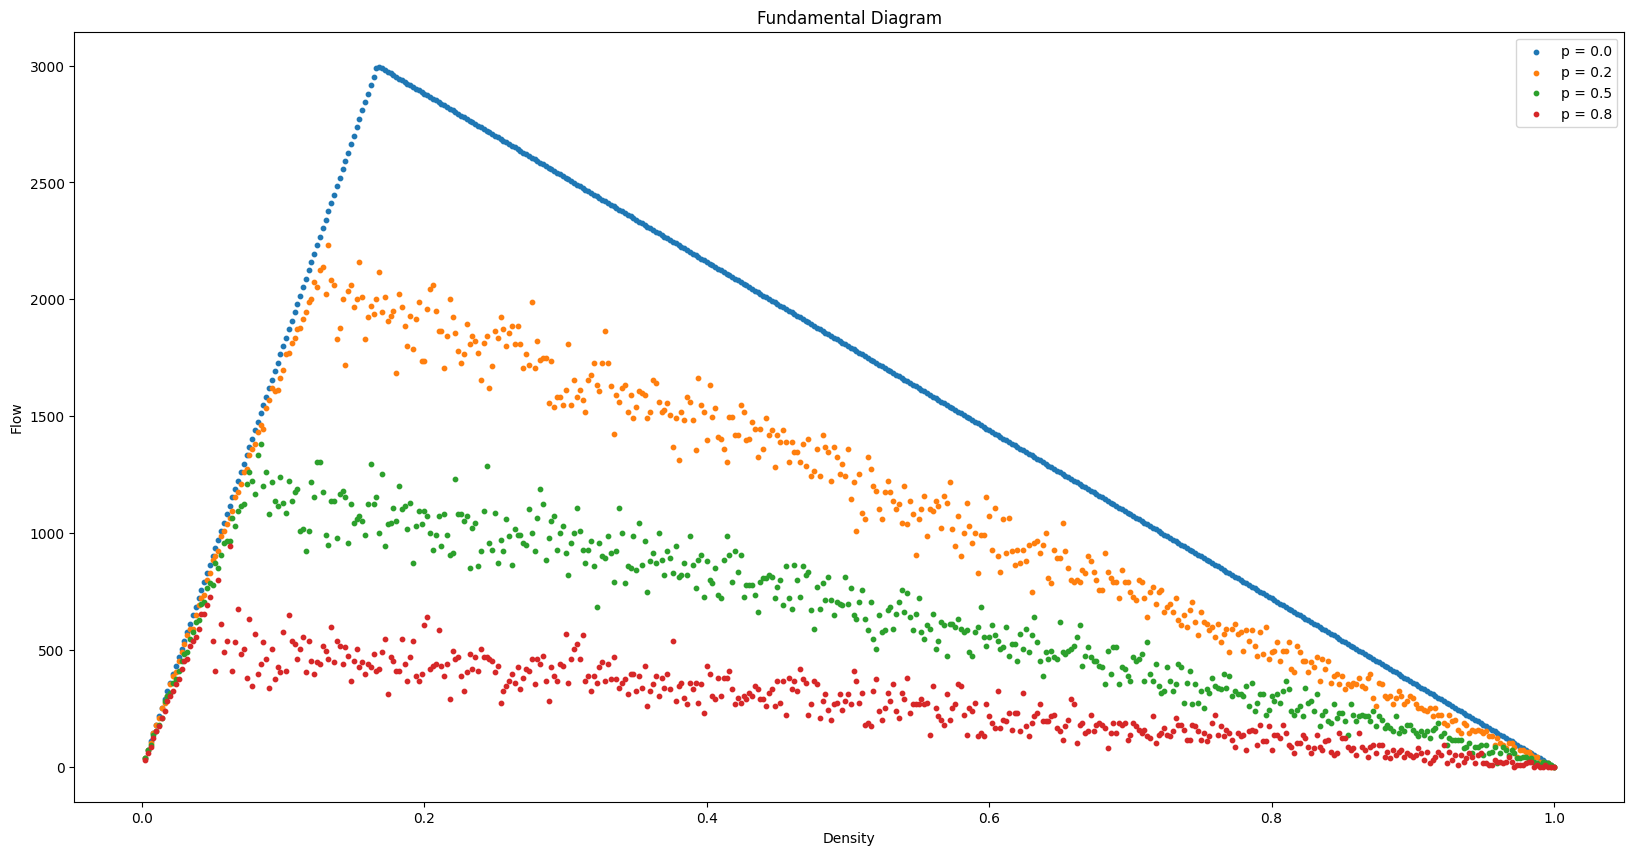
\includegraphics[width=0.8\linewidth]{assets/3.png}
\end{figure}
\newpage
With only $p=0.2$:
\begin{figure}[!h]
    \centering
    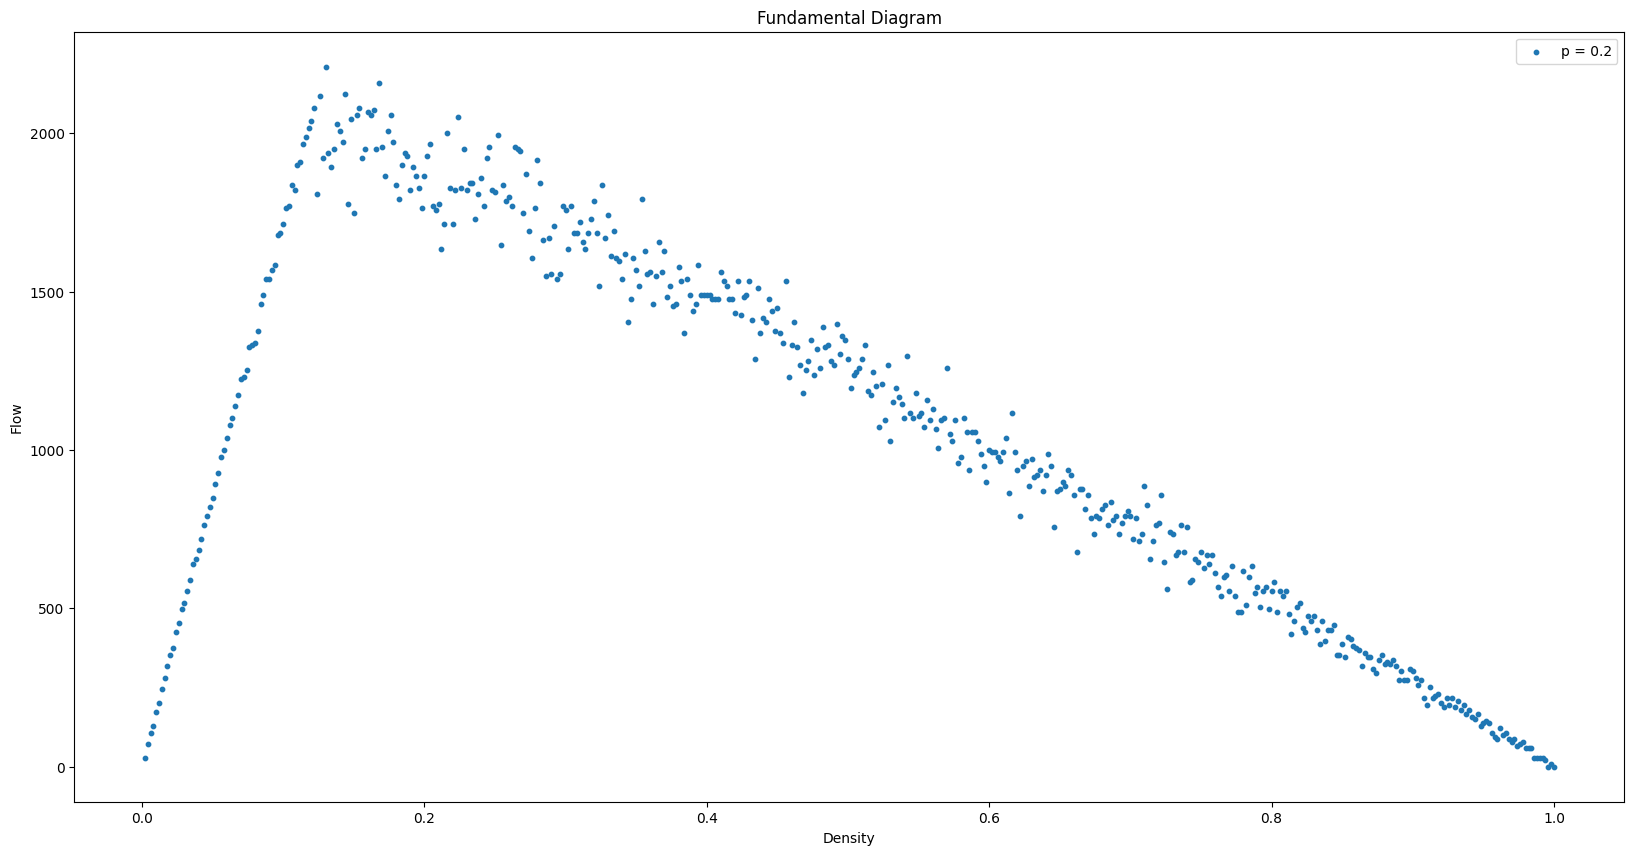
\includegraphics[width=0.75\linewidth]{assets/30.2.png}
\end{figure}

\newpage
\section{Question 1.4}
\subsection{Explanation of Algorithm}
First, we'll provide a plain English explanation of the algorithm to create a simulation of two lanes of traffic with the specified requirements in mind. The description of the algorithm is as follows: \\\\
In a two-lane traffic model, cars want to go as fast as possible without crashing. For the algorithm, we'll first initialize a data structure to track the position and speed of each car in their respective lane. We'll randomly distribute the cars with initial speeds in both lanes. For each step of the simulation, each car will speed up if it can. Cars prefer to stay in their lane and go up to the maximum allowed speed for that lane. If they're going to hit the car in front of them, they'll check if it's safe to switch to the other lane. If they can't switch safely, they slow down just enough to avoid a crash. The positions of all the cars are then updated based on these changes. After a pre-defined number of steps have been executed of the simulation, it terminates.\\\\
The algorithm requires the following inputs: length of the road (\codeword{length}), maximum speed in the left lane (\codeword{vL}), maximum speed in the right lane (\codeword{vR}), traffic density (\codeword{density}), and a randomization probability factor for dallying (\codeword{p}). The algorithm's steps are further described below: 
\begin{enumerate}
    \item 
    Initialize a two-dimensional array \codeword{road} with \codeword{length} and 2 lanes, filling with \codeword{-1} for empty cells. 

    \item
    Randomly distribute cars with initial speeds in both lanes of the road according to \codeword{density}. 

    \item
    For each time step \codeword{t} in the simulation: 
    \begin{enumerate}
        \item 
        For each car in each lane: 
        \begin{enumerate}
            \item 
            \textbf{Acceleration:} Increase speed by 1, not exceeding \codeword{vL} or \codeword{vR} respective to their lane. 

            \item 
            \textbf{Lane Inertia:} If at maximum speed, stay in the current lane. 

            \item
            \textbf{Cautious Lane Change:} If deceleration is required, check the adjacent lane for a safe lane change. A safe lane change is possible if: 
            \begin{itemize}
                \item 
                There is no car in the target space of the adjacent lane
                \item
                The next car in the adjacent lane is farther than the current speed of the given car
                \item 
                The car behind in the adjacent lane is far enough that if it accelerates, it won't reach the car's new position.
            \end{itemize}

            \item
            \textbf{Deceleration:} If a lane change isn't possible, decrease speed to avoid a collision in the current lane. 
        \end{enumerate}

        \item
        Update the positions of all the cars in the simulation based on their new speeds. 
    \end{enumerate}

    \item 
    Terminate the simulation after a pre-determined number of time steps (\codeword{num_steps}). 
\end{enumerate}

\subsection{Testing \& Verification of Algorithm}
In order to verify our simulation's efficacy, we wrote some test cases to test certain behaviors of the cars on the road. We mainly focused on ensuring that cars would accelerate to the maximum speed if there were no impediments, that cars would change lanes as expected based on the outlined requirements in the project instructions document, and that cars would preserve a higher speed (better flow) in the faster lane in a high-density scenario. The code for the test cases can be found in the accompanying Jupyter notebook for the submission, but more details on the objective and reasoning for each test case are elaborated on below. 

\subsubsection{Test Case 1}
\textbf{Objective:} To verify that a single car (in each lane) on an otherwise empty road accelerates to and maintains its maximum speed, as determined by the maximum speed settings of its lane (vL or vR). \\\\
\textbf{Why It's Good:} This test case assesses the simulation's handling of basic car dynamics, specifically acceleration. It ensures that without the influence of other cars or the need for lane changes, a car can reach and sustain the lane's maximum speed. This forms the foundation of more complex interactions and is crucial for validating the model's accuracy in simulating individual vehicle behavior.

\subsubsection{Test Case 2}
\textbf{Objective:} To check if a faster car will change lanes when approaching a slower car directly ahead, provided that a safe lane change is possible according to the simulation rules.\\\\
\textbf{Why It's Good:} This test case is pivotal for verifying the simulation's lane-changing logic, a critical aspect of two-lane traffic simulations. It tests the decision-making process of virtual drivers when encountering slower traffic and evaluates the conditions under which they opt to change lanes. This scenario is fundamental in assessing the model's capacity to simulate realistic traffic flow and prevent artificial traffic jams.

\subsubsection{Test Case 3}
\textbf{Objective:} To observe and analyze the simulation's behavior under high-density conditions, focusing on the distribution of traffic between lanes, the incidence of lane changes, and the preservation of faster flow in the designated lane (vL).\\\\
\textbf{Why It's Good:} This test case evaluates the simulation's performance under complex, dynamic conditions that closely resemble real-world traffic scenarios. It's essential for testing the model's robustness and its ability to handle congestion, lane preferences, and varying speeds realistically. This scenario helps in understanding how well the simulation can manage multiple cars interacting simultaneously, adapting to slower vehicles, and the effectiveness of the lane-changing algorithms in maintaining optimal traffic flow.

\subsubsection{Verification of Implementation}
The verification of the implementation involved running the simulation with the specified test cases and carefully observing the outcomes for each scenario. For the first two test cases, the expected behaviors were clearly defined (e.g., a car should reach a certain speed, or a lane change should occur), making it straightforward to determine whether the simulation passed or failed these tests. For the higher density behavior test, the verification was more qualitative, focusing on the overall traffic flow patterns and lane usage to assess whether they align with realistic expectations and the specified model behaviors.\\\\
In addition to observing the immediate outcomes, plotting the simulation states over time was useful for visual verification (note: in the Jupyter Notebook, there was a method in the \codeword{TwoLaneTrafficSimulation} class to generate a plot as well as a string representation printed to the console at each step of the simulation). The scatter plot display method, which visualizes the positions of cars in both lanes at each simulation step, provided clear, visual evidence of the simulation's behavior, further supporting the verification process.\\\\
Overall, these test cases are beneficial in establishing the reliability and accuracy of the two-lane traffic simulation model. They cover a broad spectrum of situations, from simple to complex, ensuring the model not only correctly implements individual vehicle dynamics but also accurately simulates the interactions and collective behaviors that emerge in two-lane traffic systems.

\subsection{Results of Experimentation}
To experiment with the two-lane traffic simulation, we created various plots varying the maximum speed of the left lane (a fast lane, like seen in highways across the U.S.), the dally factor, and the density of the traffic. We've included some of the most notable plots below, and a summary of the findings is included after the images. 

\subsubsection{Low Density, Low Dally}
\begin{figure}[!h]
    \centering
    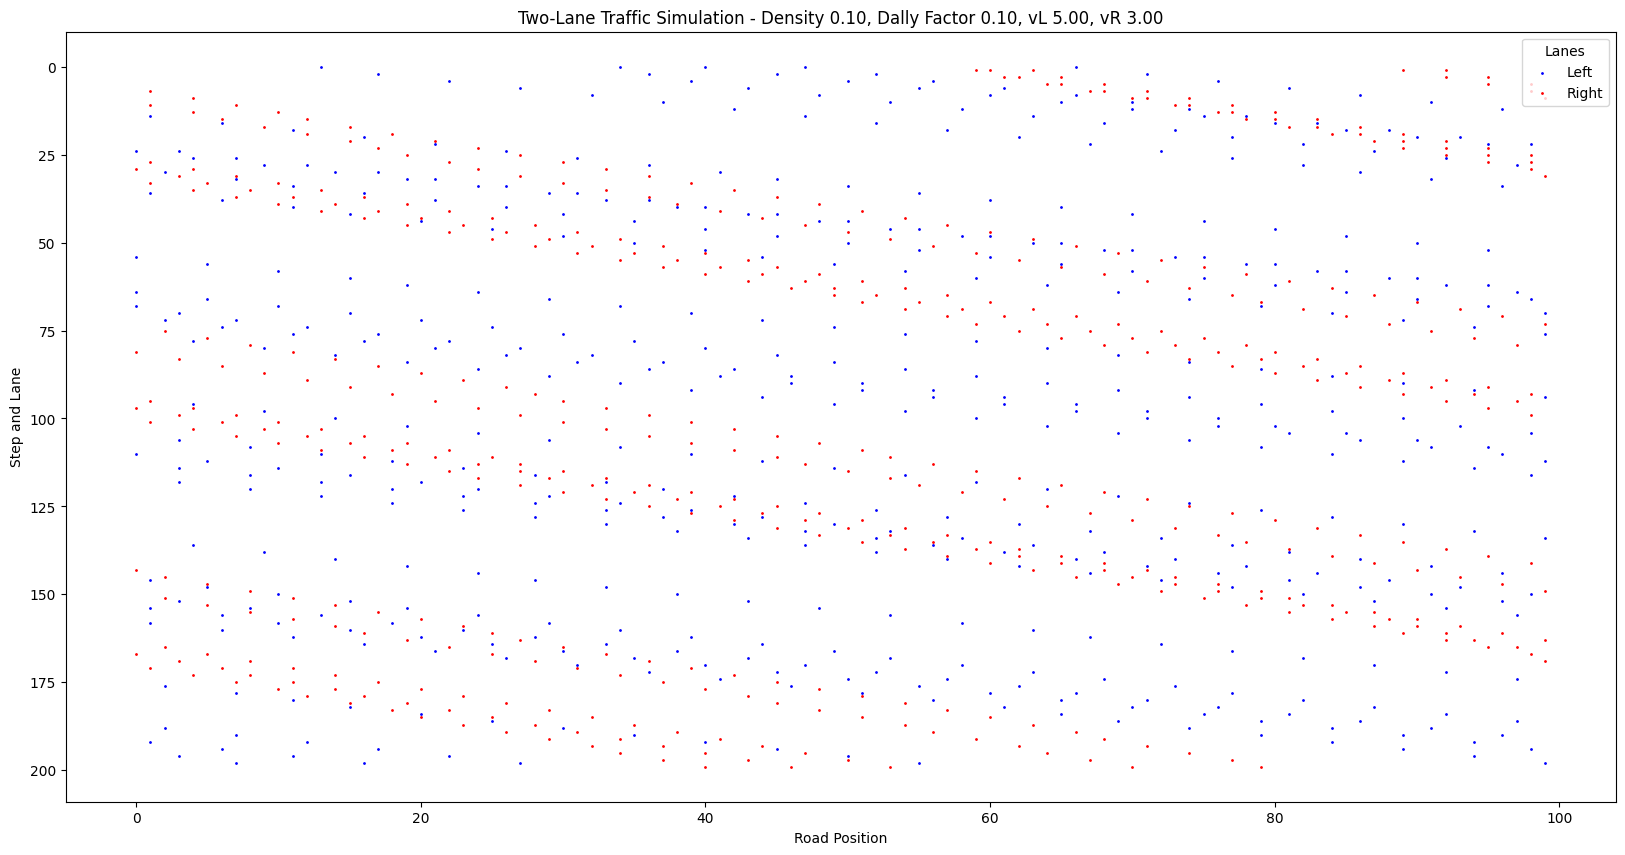
\includegraphics[width=1\linewidth]{assets/two-lane-sim-d0.1-p0.1-vl5-vr3.png}
\end{figure}

\subsubsection{Low Density, High Dally}
\begin{figure}[!h]
    \centering
    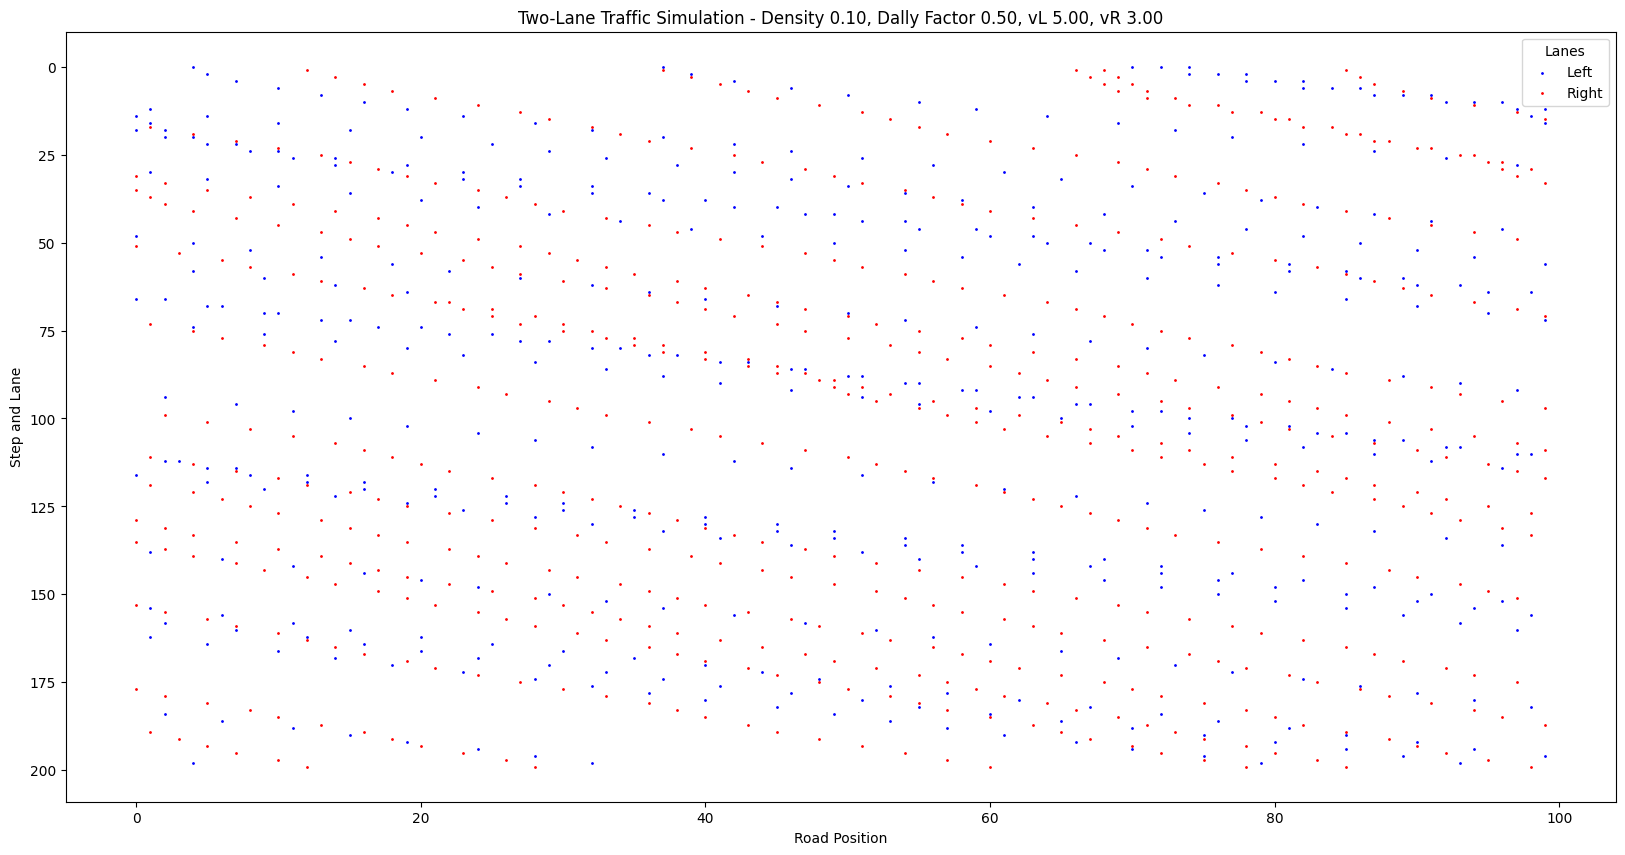
\includegraphics[width=1\linewidth]{assets/two-lane-sim-d0.1-p0.5-vl5-vr3.png}
\end{figure}

Increasing the dally factor led to slightly more buildup of traffic, as seen in the plot in 4.3.2. That said, with the low density, we don't see any major traffic jams in either plot. Cars are able to move between lanes and progress along the road without much resistance. 

\newpage
\subsubsection{Low Density, High Dally, Increased Left Lane Speed}
\begin{figure}[!h]
    \centering
    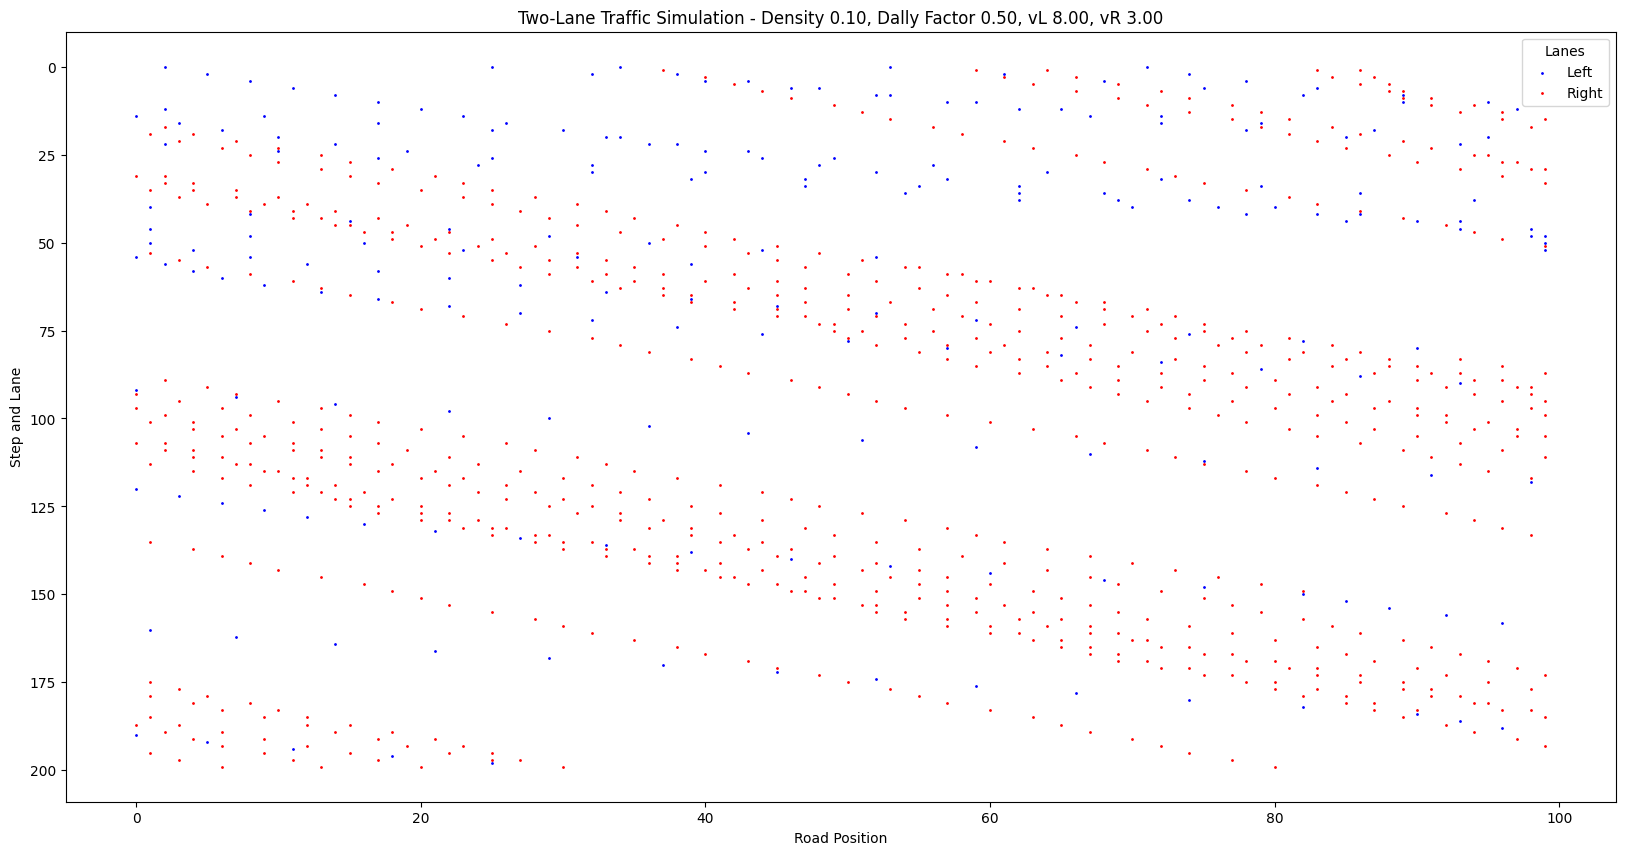
\includegraphics[width=1\linewidth]{assets/two-lane-sim-d0.1-p0.5-vl8-vr3.png}
\end{figure}

\subsubsection{High Density, High Dally}
\begin{figure}[!h]
    \centering
    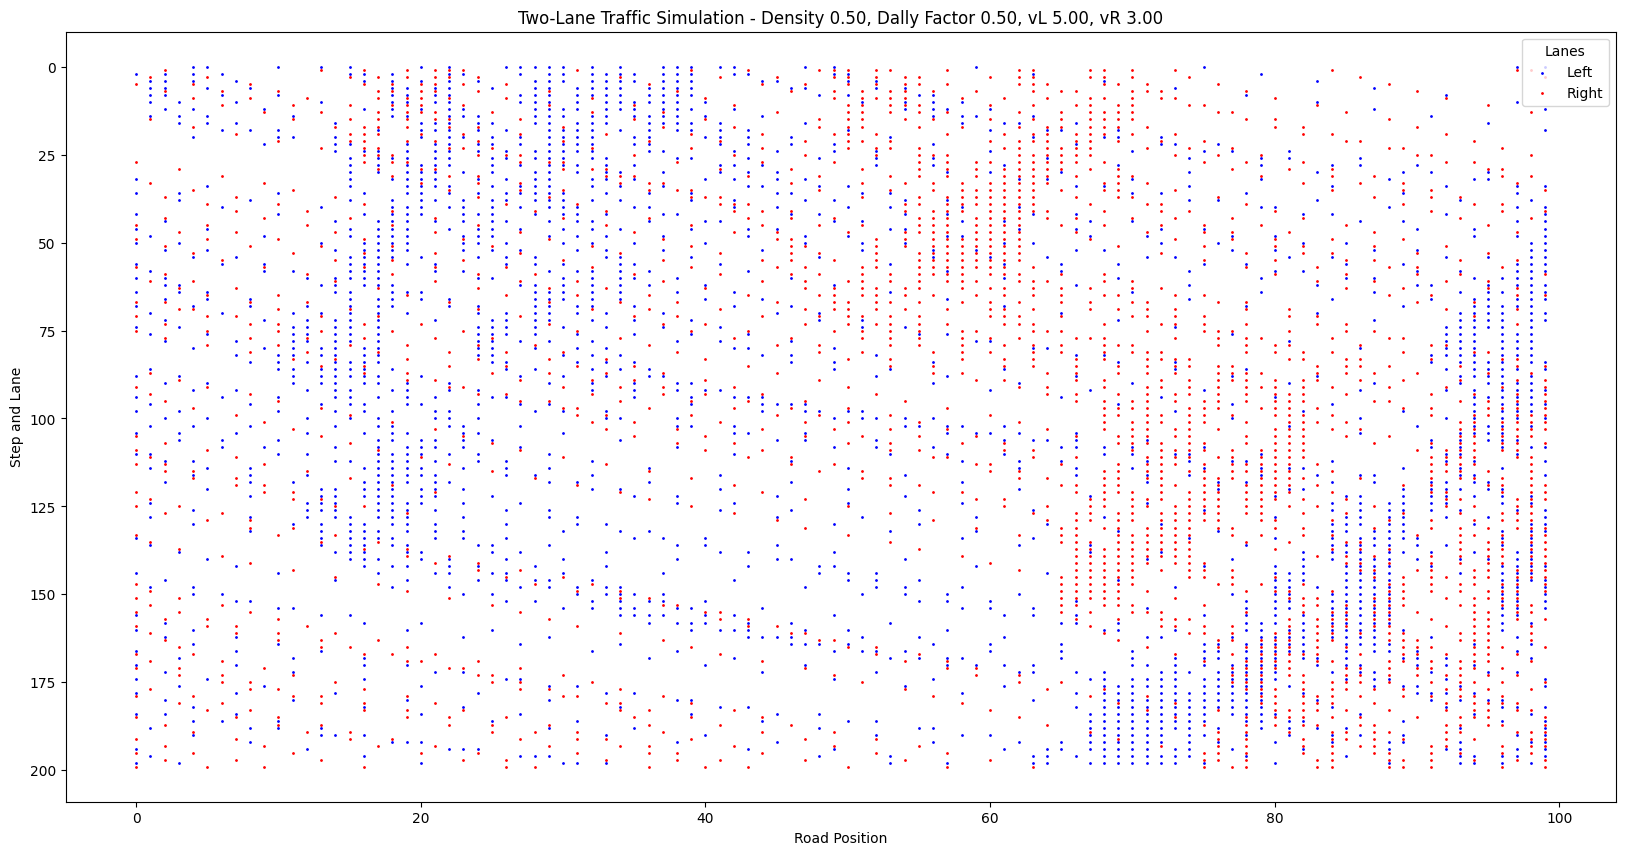
\includegraphics[width=1\linewidth]{assets/two-lane-sim-d0.5-p0.5-vl5-vr3.png}
\end{figure}

With an increase in speed in the left lane, cars were moving significantly faster, preventing major buildups in the left lane. Something interesting we observed in plot 4.3.3 was the fact that with the high dally and decreased speed, the right lane saw much more traffic as compared to the faster left lane. This is something that's witnessed on highways. With the high density, high dally, and the left lane having marginally faster speed, we begin to see more traffic buildup in both lanes in different parts of the simulation, as seen in plot 4.3.4. We also don't see buildups of traffic at the same time in the two lanes, which is quite interesting. This is also something that we might see in real life - when cars are noticing dallying and a buildup, they'll switch lanes, and then later on, that lane will face a buildup, resulting in another switch back. \\\\
Overall, we noted that there was a limitation on increasing the speed on the left lane, especially with higher densities and higher chances for dallying. This is consistent with what we'd observe in real life, as humans are more likely to dally than be the perfect driver and accelerate exactly when we'd expect - there would be numerous over-corrections that would occur, leading to traffic building up, despite the ability to reach a higher maximum speed. Another interesting observation was that with a low density, and a higher maximum speed for a fast lane, dallying could be overcome with drivers simply overtaking. That said, it would increase the density of the faster lane, and though would limit the speed of the fast lane, it would still be faster than the other lane. \\\\
We found that the two-lane traffic simulation was much more successful than previous models explored in this project, as it incorporated various driving behaviors that would be seen in real life. That said, we were limited in our scope of experimentation, and in the future, would hope to explore all the enumerations of different factors (density, dally probability, and maximum speeds for different lanes) to understand better their effects on traffic flow. Expanding and tweaking these factors can help better understand optimal conditions to prevent traffic jams, which can be incredibly useful for city planners and civil engineers alike. 

\end{document}
